%%%%%%%%%%%%%%%%%%%%%%% file template.tex %%%%%%%%%%%%%%%%%%%%%%%%%
%
% This is a general template file for the LaTeX package SVJour3
% for Springer journals.          Springer Heidelberg 2010/09/16
%
% Copy it to a new file with a new name and use it as the basis
% for your article. Delete % signs as needed.
%
% This template includes a few options for different layouts and
% content for various journals. Please consult a previous issue of
% your journal as needed.
%
%%%%%%%%%%%%%%%%%%%%%%%%%%%%%%%%%%%%%%%%%%%%%%%%%%%%%%%%%%%%%%%%%%%
\begin{filecontents*}{example.eps}
%!PS-Adobe-3.0 EPSF-3.0
%%BoundingBox: 19 19 221 221
%%CreationDate: Mon Sep 29 1997
%%Creator: programmed by hand (JK)
%%EndComments
gsave
newpath
  20 20 moveto
  20 220 lineto
  220 220 lineto
  220 20 lineto
closepath
2 setlinewidth
gsave
  .4 setgray fill
grestore
stroke
grestore
\end{filecontents*}
%
\RequirePackage{fix-cm}
%
\documentclass{svjour3}                     % onecolumn (standard format)
%\documentclass[smallcondensed]{svjour3}     % onecolumn (ditto)
%\documentclass[smallextended]{svjour3}       % onecolumn (second format)
%\documentclass[twocolumn]{svjour3}          % twocolumn
%
\smartqed  % flush right qed marks, e.g. at end of proof
\usepackage{graphicx}
\usepackage{cite}
\journalname{Requirements Engineering}
\begin{document}

\title{Network Structure and Requirements Crowdsourcing for OSS Projects}
\titlerunning{Network Structure and Requirements Crowdsourcing for OSS Projects}

%\author{Matthew Robinson \and
%    Shahram Sarkani \and 
%    Thomas Mazzuchi
%}

\author{BLINDED}

% \authorrunning{Robinson, Sarkani, and Mazzuchi} % if too long for running head
% \institute{M. Robinson \at \email{mrobinson23@gwu.edu}}

\date{Received: date / Accepted: date}
% The correct dates will be entered by the editor


\maketitle

\begin{abstract}
Crowdsourcing system requirements enables project managers to elicit feedback from a broader range of stakeholders. The advantages of crowdsourcing include a higher volume of requirements reflecting a more comprehensive array of use cases and a more engaged and committed user base. Researchers cite the inability of project teams to effectively manage an increasing volume of system requirements as a possible drawback. This paper analyzes a data set consisting of project management artifacts from 562 open source software (OSS) projects to determine how OSS project performance varies as the share of crowdsourced requirements increases using six measures of effectiveness: requirement close-out time, requirement response time, average comment activity, the average number of requirements per crowd member, the average retention time for crowd members, and the total volume of requirements. Additionally, the models measure how the impact of increasing the share of crowdsourced requirements changes with stakeholder network structure. The analysis shows that stakeholder network structure impacts OSS performance outcomes, and that the effect changes with the share of crowdsourced requirements. OSS projects with more concentrated stakeholder networks perform the best. The results indicate that requirements crowdsourcing faces diminishing marginal returns. OSS projects that crowdsource more than 70\% of their requirements benefit more from implementing processes to organize and prioritize existing requirements than from incentivizing the crowd to generate additional requirements. Analysis in the paper also suggests that OSS projects could benefit from employing CrowdRE techniques and assigning dedicated community managers to more effectively channel input from the crowd. 

\keywords{CrowdRE \and Crowdsourcing \and Collaborative Requirements Elicitation \and Stakeholder Networks \and Stakeholder Analysis}
\end{abstract}

\section{Introduction}
\label{intro}

The growing prevalence of systems with diverse and distributed stakeholders has stretched the limits of traditional stakeholder analysis techniques. These conditions make it difficult for project managers to identify an exhaustive list of stakeholders at the onset of a project. The consequent uncertainty during the stakeholder analysis process can negatively impact the quality of system requirements. To deal with this challenge, researchers have begun to develop techniques, known as crowd-based requirements processes (CrowdRE), that improve requirement quality by gathering feedback from crowds of stakeholders \cite{groen}. While CrowdRE has traditionally focused on eliciting stakeholder feedback via polls and surveys prior to the formation of requirements and marketing-driven mechanisms for prioritizing existing requirements, Glinz \cite{glinz} highlights the direct solicitation of requirements from crowds of highly-engaged stakeholders as an opportunity for the field.

Crowdsourcing requirements enables project managers to understand the range of potential use cases for a system more fully. Improved understanding of stakeholder needs translates into better system requirements and more informed prioritization decisions. Crowdsourcing, however, also has drawbacks. A high volume of requirements can overwhelm engineers and project managers \cite{groen}. Some experts \cite{snijders} have also questioned the quality of crowdsourced requirements. Understanding the trade-offs associated with crowdsourcing requirements enables projects managers to decide whether to invest in (1) incentivizing additional requirements generation from crowd members or (2) organizing and prioritizing existing requirements.

Network analysis provides a useful framework for thinking about and measuring patterns of interaction between crowd members and project contributors \cite{wood}. Past research \cite{wood, linaker} has show that stakeholder network structure can influence prioritization decisions and task completion rates. This research contends that the structure of the stakeholder network influences the effectiveness of requirements crowdsourcing and tests the following hypotheses:

\begin{enumerate}
    \item More centralized stakeholder networks result in better outcomes for OSS projects.
    \item The effect of stakeholder network structure on OSS project outcomes varies depending on the current share of crowdsourced requirements.
    \item Requirements crowdsourcing faces diminishing marginal returns.
\end{enumerate}

To test these hypotheses, this study relies on six measure of effectiveness for OSS project performance: requirement close-out time, requirement response time, comment activity, the number of requirements per crowd member, the retention time for crowd members, and the volume of requirements. Requirement close-out and response time are output measures of effectiveness, while the remainder constitute input measures of effectiveness. Statistical analysis based on a curated set of 562 open source software (OSS) projects on GitHub supports each hypothesis and concludes that OSS projects perform best when they have centralized stakeholder networks. The impact of stakeholder network structure on OSS project performance varies based on the proportion of requirements the project has already sourced from the crowd. Additionally, the study shows that the benefits of additional requirements crowdsourcing diminishes for OSS projects that already source more than 70\% of requirements from the crowd. Specifically, these projects contend with longer requirement close-out and response times, a growing backlog of unaddressed requirements, and shorter crowd retention times.

Before proceeding, readers should note several characteristics of the data set that limit the generalizability of the results. First, this research considers OSS projects. Proprietary software and physical products face different challenges. Insights about crowd engagement in an OSS context do not necessarily transfer. Second, since crowd members in an OSS context are software developers, they have greater expertise than a typical crowd. A less technical crowd may lack the experience necessary to effectively generate requirements. Third, the OSS projects in the data set consist of a curated set of active, community-led projects that have not suffered substantial attrition amongst core contributors. Drawing conclusions about OSS projects more broadly would require consideration of how stakeholder network structure changes over team. Finally, since the data set only considers active OSS projects, the results do not apply to OSS projects that have not progressed beyond the system design phase.

This paper begins by reviewing the literature on crowd-based requirements processes, stakeholder networks, and open-source software systems. The methodology section details the data set, explains the experimental design, justifies each modeling decision, and highlights potential drawbacks. The results section presents the regression models and associated diagnostics. The paper concludes by interpreting the results, discussing limitations, and suggesting avenues for future research.

\section{Literature Review}
\label{litreview}

This research addresses three distinct but related aspects of requirements engineering: crowdsourcing, CrowdRE, and collaborative requirements elicitation. Crowdsourcing refers to the process of outsourcing of tasks to a crowd of contributors \cite{howe, howe2}. In this case, OSS projects outsource requirements generation to crowds of developers. CrowdRE automates the analysis of stakeholder feedback \cite{groen}. This research leverages CrowdRE to study the effect of crowd participation on OSS projects and suggests when OSS project managers should consider employing CrowdRE techniques. Finally, collaborative requirements elicitation and related research on stakeholder communities provides a theoretical basis for the application of network analysis within the domain of requirements engineering. The literature review begins, however, with a brief overview of existing research on requirements engineering for OSS projects.  

\subsection{Requirements Engineering for OSS}
\label{oss_re}

The OSS ecosystem consists of a diverse array of projects. Camara and Fonseca \cite{camara} identify four categories of OSS projects---community-led, corporate-led, academic-led, and innovation-led---each of which approaches the requirements process differently. Scacchi \cite{scacchi} describes the requirements process for community-led OSS projects as less formal, with requirements often arising from discussion forums rather than through rigorous stakeholder analysis. This process works for OSS because most OSS users are developers. As a result, empirical research \cite{kuriakose, paech} shows that OSS users have an unusually strong understanding of the underlying technical details of an OSS project and can formulate reasonably high quality requirements without needing a product manager as an intermediary. This research considers crowds of technically skilled developers who generate requirements for community-led OSS projects.

Several researchers have developed frameworks for assessing OSS project performance. Stewart and Gosain \cite{stewart} differentiate between input and output measures of effectiveness. Input measures of effectiveness include the attraction and retention of developers, while output measures of effectiveness consider factors such as task completion rates and software quality \cite{stewart}. Crowston and Howison \cite{crowston} and Ghapanchi, et al. \cite{ghapanchi} cite task completion rates, code quality, user satisfaction, developer satisfaction, and contributor turnover rate as key indicators of success for OSS projects. Ma \cite{ma} addresses the requirements process more directly and points to the volume of user feedback and the level of agreement between different sets of users on prioritization as outcomes project managers should consider. This study borrows elements from the existing literature on OSS performance measurement to determine how stakeholder network structure and requirements crowdsourcing impact OSS project outcomes.

\subsection{Crowdsourcing}
\label{crowdsourcing}

Howe \cite{howe, howe2} introduced the concept of crowdsourcing as the process of outsourcing tasks to a network of contributors through an open call for participation. As examples of crowdsourcing, Howe cites corporations soliciting research and development ideas through prize competitions on platforms such as Innocentive \cite{howe} and the use of tools such as Amazon Mechanical Turk to complete data labeling tasks \cite{howe}. Expanding on Howe's work, Brabham \cite{brabham, brabham2} distills the concept of crowdsourcing into four essential elements: 

\begin{itemize}
    \item An organization with a task to perform
    \item A crowd of participants willing to perform the task
    \item An online tool to coordinate the performance of the task
    \item Mutual benefits for the crowd and the organization
\end{itemize}

Under this definition \cite{brabham}, the crowd includes anyone outside the organization soliciting the task. This paper considers crowd-generated requirements in OSS projects. Crowdsourcing requirements for OSS projects meets all four of Brabham's \cite{brabham} criteria for crowdsourcing. In an OSS project, requirements generation is the task, the core contributors constitute the organization, users represent the crowd, and online code repositories facilitate task completion. Although OSS projects do not explicitly reward crowd members when they submit requirements, both parties still benefit. The OSS project team receives feedback, which they use to improve the tool. In return, crowd members benefit from a more useful and reliable dependency for their own software projects. Crowdsourcing, therefore, provides a useful framework for understanding the solicitation of requirements from the crowd in OSS projects.

With the emergence of adequate tools, crowdsourcing has grown more prevalent, particularly in the field of software engineering. According to Mao, Capra, Harman, and Jia  \cite{mao}, published research on crowdsourcing within the software engineering domain grew from only one paper in 2008 to over 200 in 2015. Writing in 2015, LaToza and Van Der Hoek  \cite{latoza} note the rise of several crowdsourcing modalities within the software engineering community, including peer participation, competitions, and micro-tasking. Treatment of the topic within the context of software engineering, however, has primarily focused on implementation. Although Stol, LaToza, and Bird \cite{stol} argue that crowdsourcing facilitates quicker identification of bugs and more productive feedback, they do not discuss the implication of these outcomes for stakeholder analysis more broadly.

Although the literature has largely focused on implementation, Glinz \cite{glinz} suggests that project managers can also crowdsource system requirements. Gerth, Burnap, and Papalambros \cite{gerth} concur, but argue that while crowdsourcing can improve the quality of requirements under the right circumstances, crowdsourcing only produces these benefits if project managers institute well-governed processes for managing the crowd. Optimizing these processes presents challenges for project managers because different use cases and crowd sizes demand different approaches \cite{gerth}. This research examines the impact stakeholder network structure has on the trade-offs associated with crowdsourcing requirements and argues that OSS project managers should adopt different strategies for managing the crowd depending on the specific circumstances of the project.

\subsection{Crowed-Based Requirements Engineering}
\label{crowd_based_re}

Expanding on the notion of crowdsourcing, the requirements engineering community has developed crowd-based requirements engineering (CrowdRE) \cite{groen}, which applies automated methods to mine insight from anonymous crowd feedback. CrowdRE \cite{groen} enables project managers to efficiently identify the needs of a diverse set of stakeholders without having to interact with each crowd member individually. Soliciting crowd feedback improves product quality because, as research on Market Driven Requirements Engineering \cite{regnell} points out, OSS serves an open market of users rather than a fixed set of customers. Hosseini, Phalp, Taylor, and Ali \cite{hosseini} suggest a host of additional benefits, including nimbler adaptation of requirements to changing conditions, empirical validation of assumptions about the OSS project, and the identification of new stakeholders and use cases. CrowdRE benefits users because crowd feedback results in a more functional and reliable product \cite{groen}.

According to Khan et al. \cite{khan}, three concepts underlie the basic theory of CrowdRE: the crowd, the task, and the mechanism. Khan, et al. \cite{khan} define the crowd as the set of entities engaged in the requirements process and categorize crowds according to their scale, role, and level of expertise. Wang, et al. \cite{wang} further differentiate between explicit user feedback, which crowd members actively contribute, and implicit user feedback based on observing user activity. This research considers explicit feedback from crowds of developers with high levels of expertise. As noted throughout this paper, the results do not generalize to other types of crowds. Non-expert crowds, for instance, may not have a deep enough understanding of a system to generate quality requirements.

To unlock the benefits of CrowdRE, project managers must provide crowd members with an incentive to participate \cite{groen}. Snijders and Dalpiaz \cite{snijders, snijders2} suggest using gamification to motivate crowds. In exchange for participation, crowd members gain social standing within the community \cite{snijders, snijders2}. Levy, Hadar, and Te'eni \cite{levy} propose an alternative solution that starts with micro-crowds and fosters connections between micro-crowds as the project matures. According to Levy, Hadar, and Te'eni \cite{levy}, the micro-crowd approaches increases user satisfaction and produces higher quality requirements \cite{levy}.

In addition to applying CrowdRE by automatically mining user feedback, this research explores the conditions under which OSS projects benefit most from CrowdRE. Namely, this research offers a framework that helps OSS project managers determine under what circumstances they should incentivize additional crowd participation, and when they should focus on organizing and prioritizing existing crowd engagement. 

\subsection{Collaborative Requirements Elicitation and Stakeholder Networks}
\label{network_re}

Collaborative requirements elicitation \cite{stakerare, stakenet, stakesource, mobasher} uses social networks to identify new stakeholders, organize the input of existing stakeholders, and prioritize requirements based on common needs. In addition to providing a basis for the use of social networks for requirements engineering, the collaborative requirements elicitation literature develops an approach to structuring a large volume of feedback from the crowd. Lim, et al. \cite{stakerare, stakenet, stakesource, lim} suggest using network structure and collaborative filtering to group and prioritize requirements. Mobasher and Cleland-Huang \cite{mobasher} use recommendation systems to accomplish the same end. In addition to drawing inspiration from the use of social networks in the collaborative requirements elicitation literature, this study suggests opportunities to employ these techniques in an OSS setting.

Related research has focused on how network structure influences social dynamics within a project. Wood, Sarkani, Mazzuchi, and Eveleigh \cite{wood} build networks based on shared interest in a system component to identify lines of influence within stakeholder groups. Lopez-Fernandez, et al. \cite{lopez} apply stakeholder analysis to identify key influencers amongst stakeholders in OSS projects within the Apache ecosystem. Linaker, Regnell, and Damian \cite{linaker} show that stakeholders who occupy central positions within a network more strongly influence the priorities of OSS projects. Separately, Damian, Marczak, and Kwan \cite{damian} use social networks to show that physical distance does not limit the ability of remote software development teams to collaborate effectively on requirements. Toral, Martinez-Torres and Barrero \cite{toral} demonstrate that higher levels of network concentration improves information flow within threaded discussions linked to OSS requirements. Kluender, et al. \cite{kluender} formulate a mathematical approach based on network centrality to characterize communication distance within networks of collocated software developers, concluding that greater communication distance increases the likelihood of social conflicts.

A final line of inquiry evaluates the relative effectiveness of different stakeholder network topologies. Iyer and Lyytinen \cite{iyer} show that OSS projects with more centralized communications structures have higher task completion rates. The advantage of centralizing, however, diminishes as requirement volume increases \cite{iyer}. For projects that contend with a high volume of requirements, they recommend decentralized project management processes \cite{iyer}. This research validates existing studies, which broadly show that projects with more concentrated stakeholder networks achieve better outcomes, and extends the current understanding of the topic by demonstrating that the effect of stakeholder network structure on OSS project performance changes depending on the proportion of crowdsourced requirements.

\subsection{Research Contribution}
\label{contribution}

This research has both practical and scientific implications. From a practical standpoint, this research suggests that, beyond a certain point, OSS projects benefit more by implementing procedures that channel existing crowd engagement more effectively than by incentivizing additional requirements generation. Within the framework of CrowdRE, this means emphasizing gamification \cite{snijders, snijders2} while the proportion of crowdsourced requirements remains low and automated requirements triage methods \cite{stakesource, mobasher} as the share of crowdsourced requirements rises. Furthermore, OSS projects could benefit from assigning a team member to focus exclusively on engaging with the crowd and managing requirements, enabling the rest of the team to concentrate on implementation.

From a scientific perspective, this paper makes several contributions. First, applying CrowdRE for requirements generation within an OSS context is novel \cite{glinz}. In addition to applying CrowdRE, this research suggests circumstances under which OSS project managers would benefit from CrowdRE. Second, the paper shows that requirements crowdsourcing faces diminishing marginal returns. That is, beyond a certain level of crowd engagement, the overhead of managing limits the degree to which an OSS project benefits from that engagement. This observation does does not currently exist in the literature. Third, this research adds to the existing discussion \cite{groen, levy, hosseini, snijders, snijders2} on crowd motivation. Namely, it suggests that project managers should not only consider how, but also when to motivate additional crowd participation. Fourth, the paper shows that stakeholder network structure has a significant impact on OSS project performance. Finally, this study uses empirical analysis to confirm several claims within the CrowdRE literature \cite{glinz}, further cementing crowd engagement as an important construct for thinking about the requirements process.

\section{Methodology}

To evaluate how the effect of increasing the share of crowdsourced requirements changes with network structure, the research team employs the following procedure:

\begin{enumerate}
    \item Build stakeholder networks from project management data.
    \item Measure the share of crowdsourced requirements for each project.
    \item Train regression models to estimate the effect requirements crowdsourcing and stakeholder network structure has on measures of effectiveness for OSS project performance.
    \item Interpret the results.
\end{enumerate}

The methodology section begins with a detailed description of the data set and then defines the input variables for the regression models. Inputs to the regression models include the share of crowdsourced requirements, network structure variables, project management measures of effectiveness, and several control variables. Finally, the section outlines the statistical analysis framework, which uses generalized linear models.

\subsection{Data Set}
\label{data_set_section}

This research leverages publicly available project management data from GitHub, a widely used code repository and collaboration tool. In total, the data set consists of 562 packages from a curated list of OSS projects and includes 24,730 distinct users, 34,982 issues, and 165,836 comments. Of the 24,730 distinct users, 1,954 submitted issues to multiple projects and 81 users submitted issues to more than 5 projects. Only 9 users submitted issues to more than 10 projects. Within the data set, 5,607 users contributed code to at least one project and 390 contributed code to multiple projects. No user contributed code to more than 10 projects.

The curated list of projects originated from community maintained repositories containing links to popular packages for the five most commonly used programming languages: C++ \cite{cpp}, Java \cite{java}, JavaScript \cite{javascript}, PHP\cite{php}, and Python\cite{python}. The research team used the GitHub application programming interface in June 2019 to download project management data for each project. Since the analysis depends on having enough information to build a meaningful stakeholder network, the data set only includes projects that have at least thirty requirements.

GitHub projects manage requirements through issues. Collaboration on issues occurs through comments. Issues and comments also serve as documentation. GitHub tracks both tasks and pull requests as issues. The analysis excludes pull requests because pull requests reflect contributions to the code base rather than requirements. GitHub issues present additional difficulty because, in some cases, issues function as a help forum rather than a project management artifact. Fortunately, GitHub provides labels to separate questions from tasks. To limit the analysis to project requirements, the data only includes issues with the labels “bug”, “change”, “enhancement”, “feature”, “feature request”, or “suggestion” and ignores issues with the labels “documentation”, “help wanted”, and “question”. Although GitHub allows users to create custom labels, the analysis discards them because most custom labels appear in only a single project.

\subsection{Crowdsourced Requirements}

The crowdsourcing literature \cite{howe, howe2, brabham, brabham2} conceives of a crowd as a group of individuals outside an organization who perform a defined task in exchange for a reward. While all contributors in an OSS setting---including core developers---constitute a crowd in a colloquial sense, they vary with respect to their degree of participation. Setia, et al. \cite{setia} define several categories of contributors. Core contributors implement code, manage requirements, and review code contributions from peripheral contributors. In addition to using an OSS package, peripheral contributors suggest and implement new features, find and fix bugs, and promote product adoption \cite{setia}. Setia, et al. \cite{setia} differentiate between high engagement peripheral contributors who implement features and fix bugs from low engagement peripheral contributors who identify requirements, but do not contribute directly to the code base \cite{setia}. Finally, non-contributors use the software package but do not engage directly in the software development process \cite{setia}.  

Within the context of this paper, the crowd refers to a set of low engagement engagement peripheral stakeholders, who identify requirements and suggest new features but do not contribute to the code base. Note that this definition does not constitute a crowd in the traditional sense. Howe \cite{howe} originally conceived of crowdsourcing as an exchange---crowd members perform a task in exchange for a reward. Here, crowd members do not earn an explicit reward for providing feedback. However, they still have an incentive to improve product quality. The implicit reward is a more functional open source dependency for their own projects. Since peripheral contributors would have no reason to surface requirements without this incentive, the solicitation of requirements for OSS projects conforms to the prevailing definition of crowdsourcing. Further, this notion aligns with the conception of the crowd in CrowdRE \cite{groen}, which envisions a mutually beneficial relationship between crowd members and the project team and conceives of a certain type of crowd member---impact seekers---who view the implementation of their suggestions as a primary motivator. Hereafter, the term crowd members will refer to low engagement peripheral stakeholders in OSS projects, who generate requirements but do not contribute code.

Certain team members, such as dedicated project managers, may introduce requirements without ever writing code for an OSS project. This risks misclassifying requirements that the project manager has developed as crowd-contributed requirements, even though they originated from the project team. While software development teams in professional settings typically employ dedicated product managers, in the OSS community developers manage most projects. An analysis of the data set bears this out. Of stakeholders with a non-negative betweenness centrality---those who serve as a bridge to other stakeholders---81\% have contributed code to a project, as have 95\% of those with a betweenness centrality greater than $0.1$. Therefore, conflation of crowd and project manger contributed requirements does not present a concern for the OSS projects in this data set.

Of contributors with a betweenness centrality greater than $0.1$, 81\% have commented on a requirement within a year of the collection date, indicating that (1) the projects remain active and (2) critical nodes represent active members of the community. This reflects the fact that the OSS project sample comes from a curated list of active projects. A random sample of community-led OSS projects may not share this characteristic, especially if the data set contains a high proportion of stale projects, limiting the applicability of the results to OSS projects more broadly.

\begin{figure*}
  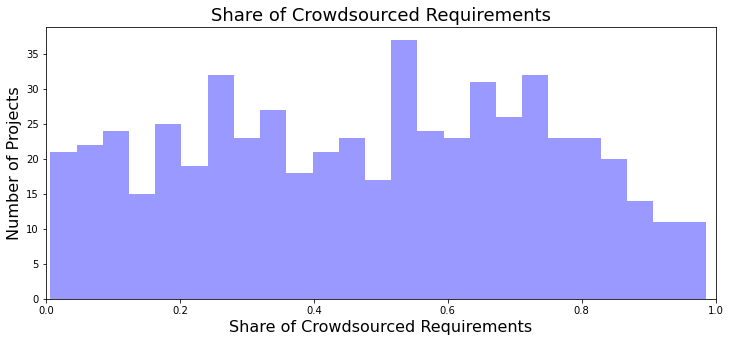
\includegraphics[width=0.95\textwidth]{crowd_pct_hist.png}
\caption{Percentage of crowdsourced requirements in the data set.}
\label{crowd_pct_hist}
\end{figure*}


A histogram of the share of crowdsourced requirements appears in Figure \ref{crowd_pct_hist} and reveals an approximately uniform distribution across the entire range of values. On average, projects in the data set sourced 48\% of requirements from the crowd. The wide distribution for the proportion of crowdsourced requirements underscores the diversity of project management strategies for OSS projects and makes the data set ideal for comparing their relative effectiveness. The data includes some projects that do not crowdsource any requirements, which enables the analysis to test against a baseline in which no crowdsourcing occurs.


\subsection{Network Analysis}

\subsubsection{Constructing Networks}
\label{network_section}

The stakeholder networks in this study consist of undirected, unweighted graphs where nodes represent stakeholders and edges represent spontaneous collaboration on a requirement. As noted in Section \ref{data_set_section}, the stakeholders in the data set only include contributors and users who have submitted requirements. Using the definition from Mitchell, Agle, and Wood \cite{mitchell}, this constitutes a narrow stakeholder set because it excludes stakeholders who do not directly participate in the requirements process. In this case, the network reflects not only a narrow stakeholder set, but also an expert stakeholder set, because most crowd members for an OSS project are developers themselves. Of course, concentric circles of stakeholders exist beyond this core group, including users who have not submitted requirements, developers of dependent packages, and the broader community for a programming language. Since this study focuses on the requirements process, excluding peripheral stakeholders does not materially affect the results. Additionally, limiting analysis to available data about the crowd conforms to standard practice within CrowdRE \cite{khan}. The appendix contains additional detail on about the procedure for constructing the stakeholder networks.

\subsubsection{Measuring Network Structure}
\label{network_structure}

This study uses three metrics to measure network structure: the Gini coefficient for network concentration, average minimum path for network breadth, and the clustering coefficient for the level of localized clustering. These numerical measures produce more information than categorical measures of network structure and make the resulting models more useful in a project management context. Project managers do not have enough control over a stakeholder network to change its structure from one broad category to another. However, they can implement strategies that nudge the structure of the network in a particular direction. As a result, project managers benefit more from an understanding of the impact of smaller changes in network structure. Numerical measures capture these changes better than categorical variables.

The Gini coefficient \cite{gini, gini2}, which ranges from zero to one, measures the amount of inequality in the degree distribution of the nodes and characterizes the level of concentration in the network. A Gini coefficient of zero reflects perfect equality and one represents perfect inequality. Although typically applied in the context of income inequality \cite{gini2, yitzhaki}, Toral, Martinez-Torres, and Barrero \cite{toral} show that the Gini coefficient also provides a useful measure of concentration in contributor networks for OSS projects. The appendix provides additional details on the procedure for calculating the Gini coefficient.

The average minimum path \cite{holland} measures the dispersal of the network. Computing this metric involves finding the minimum path between each pair of nodes in the network and taking the simple mean of the resulting minimum paths \cite{holland}. The clustering coefficient \cite{holland}, which calculates the probability that two incident nodes will form a triangle and takes values between zero and one, serves as a measure of the degree of localized clustering in a network. Networks with a low level of localized clustering have hub-and-spoke structures, whereas networks with substantial localized clustering look more like webs.

Adding nodes or edges to a network changes all three network structure variables simultaneously. To capture this relationship, the regression models include interaction terms between the network structure variables. To understand how the impact of requirements crowdsourcing changes with network structure, the models also include interaction terms between each network structure variable and the share of crowdsourced requirements. Interpreting the coefficients on these variables enables project managers to determine under what conditions they should consider promoting additional crowdsourcing.

\subsection{Measures of Effectiveness}
\label{measures_of_effectiveness}

The dependent variables in this study represent OSS project measures of effectiveness and derive from the measures Stewart and Gosain \cite{stewart}, Crowston and Howison \cite{crowston}, Ghapanchi, et al. \cite{ghapanchi}, and Ma \cite{ma} discuss in their respective work. Table \ref{variable_table} details the six measures of effectiveness in this study: requirement close-out time, requirement response time, comments per requirement, requirements per crowd member, crowd retention time, and requirement volume. 

Stewart \cite{stewart} describes task completion rate as an output measure of effectiveness for OSS projects. Project teams close out a requirement when they either (a) implement the requirement or (b) decide not to address it. Since either outcome provides feedback to the crowd member who submitted the requirement, both reflect strong engagement from the project team. In this data set, requirement close-out time measures the average number of days between the opening and closing of a requirement and only considers requirements that the project team has closed. Requirement response time captures the average number of days between the opening of the requirement and the initial response to the requirement, either by commenting on or closing the requirement. While Stewart \cite{stewart} does not discuss requirement response time as an output measure of effectiveness, this variable builds a stronger understanding of the level of engagement from the project team and also impacts input measures of effectiveness, such as user retention. If members of the project team do not respond in a timely manner, crowd members may not continue to contribute requirements.

\begin{table}
\caption{Measures of Effectiveness}
\label{variable_table}
\begin{tabular}{llllll}
\hline\noalign{\smallskip}
Variable & Category & Description  \\
\noalign{\smallskip}\hline\noalign{\smallskip}
Requirement Close-out Time & Output & Average time in days between requirement \\
&& submission and close-out. \\
Requirement Response Time & Output & Average time in days between requirement \\
&& and the project team's response \\
&& to the requirement\\
Comments Per Requirement & Input & The average number of comments on \\
&& each requirement. \\
Requirements Per Crowd Member & Input & The number of requirements \\
&& each crowd member has submitted.\\
Crowd Retention Time & Input & The time in days between the \\ 
&& first and last requirements a crowd \\
&& member submits. \\
Requirement Volume & Input & Total number of requirements divided \\
&& by project age in years.\\
\noalign{\smallskip}\hline
\end{tabular}
\end{table}

Per Stewart's \cite{stewart} taxonomy, the remaining dependent variables reflect input measures of effectiveness. The following three variables measure levels of crowd engagement within OSS projects. Comments per requirement indicates the average number of replies in threaded discussions about a requirement. Requirements per crowd member captures the average number of requirements a crowd member submits over the lifetime of the project. Retention time finds the average span, in days, between the initial and final activity on a project by a crowd member. For each of these variables, higher values represent positive outcomes.

Requirement volume divides the total number of project requirements by the age of the project in years. Scaling by project age allows for a more accurate comparison of projects that started at different times. Increasing the volume of requirements can represent either a positive or a negative outcome, depending on the situation. On the one hand, a higher volume of requirements enables project managers to process feedback from a broader range of stakeholders \cite{hosseini}. However, an excessive number of requirements can overwhelm project teams \cite{groen}, lower the average quality of requirements \cite{groen}, and make prioritization difficult \cite{stakerare, stakenet}. Therefore, requirement volume requires additional context from the other variables to determine whether it helps or hurts.

Although these variables reflect many of the  measures of effectiveness in the literature, several remain unaddressed. The data set does not capture software quality \cite{stewart}, developer satisfaction \cite{ghapanchi}, user satisfaction \cite{ghapanchi}, the quality of requirements \cite{ma}, or the level of agreement between users about requirements \cite{ma}. While in some circumstances \cite{pagano} the length of the requirement can serve as a proxy for its quality, in this case it cannot. For instance, a measure based on length would characterize a bug report that contains a long error message with no additional information as a high quality requirement, when in reality it is not. Conversely, including important information such as version numbers and system information does not add considerably to the length of the requirement, but greatly increases its quality.

Additionally, this study focuses only on requirements elicitation and does not consider other aspects of the requirements process, such as prioritization. Addressing prioritization is difficult because ambiguity about whether a project team has implemented or dismissed a requirement makes the relative priority of requirements difficult to discern. While strategies exist to address this issue---for instance, searching for linked pull requests---the research team kept prioritization of individual requirements out of scope to limit complexity. Moreover, the GitHub data set does not contain any information from the system design phase. Consequently, the results of this study only apply to active OSS projects that have already advanced beyond the system design phase.

\subsection{Regression Analysis}

\subsubsection{Generalized Linear Models}
\label{glm}

The analysis utilizes generalized linear models (GLMs) in the case of non-normal response variables and ordinary least squares (OLS) regression in the case of normal response variables to estimate the magnitude of the effect of network structure and requirements crowdsourcing on each measure of effectiveness. Using GLMs enables the research team to account for the complexities of the data, including non-normality, while still producing interpretable results amenable to statistical hypothesis testing.

For normal response variables, the team performs linear regression using OLS. Elsewhere, the GLMs assume a Gamma distribution because each measure of effectiveness has a strictly positive domain. In the regression analysis the research team uses a p-value of $0.05$ to determine statistical significance. To validate the distribution assumption, the research team computes maximum likelihood estimates using the data for the response variables and then performs a Kolmogorov-Smirnov (KS) goodness-of-fit test \cite{wackerly, massey}. Using the log link function, the most common link function for Gamma regression \cite{fahrmeir}, the regression model has the following form.

\begin{equation}
\label{gamma_glm}
    E[Y|X] = e^{\alpha + X \beta}
\end{equation}

Computing the marginal effect of each independent variable requires taking the derivative of Equation \ref{gamma_glm}, which appears below in Equation \ref{gamma_marginal}.

\begin{equation}
\label{gamma_marginal}
\frac{\partial E[Y|X, x_i]}{\partial x} = \beta_i \times e^{\alpha + X \beta}  = \beta_i \times \hat{y}
\end{equation}

Note that, for Gamma regression, the marginal effect depends on the values of the independent variables. As a result, unlike in OLS, each observation has a different marginal effect. Computing a representative measure for the marginal effect of a variable requires either (a) averaging the marginal effects across observations or (b) computing the marginal effect at typical values for the independent variables. In this case, the interaction between the network structure variables makes it difficult to choose sensible representative values. As a result, the research team decided to average the marginal effects across observations.

\subsubsection{Model Specification}

The research team used automated variable selection to mitigate against the risk of overfitting. Specifically, the models employ the hybrid stepwise variable selection technique outlined in Friedman, Hastie, and Tibshirani \cite{friedman, derkson}. This variable selection technique begins with a linear regression model that contains only the intercept. On each subsequent step, the method considers the addition or deletion of a variable in the model and stops when no addition or deletion would improve the Akaike Information Criteria (AIC) of the model \cite{friedman}. In addition to the variables of interests the analysis includes project age, the number of contributors, the number of crowd members, and the number of requirements as control variables to improve inference and mitigate against attenuation bias for the variables of interest.

\subsection{Trade-off Analysis}
\label{trade-off}

The regression models described in Section \ref{glm} provide project managers with the capability of exploring the trade-off space between various measures of effectiveness \cite{parnell}. As noted in Section \ref{network_structure}, while project managers cannot dramatically change the structure of the stakeholder network, they can affect smaller changes in the stakeholder network by adjusting their crowd engagement strategy. Therefore, from a practical perspective, project managers face a menu of options, which represent outcomes associated with crowd participation rates that fall within a narrow band of the current level. The research team devised the following methodology to estimate the trade-off space:

\begin{itemize}
    \item For each covariate in each regression model, find the values associated with the current state of the OSS project.
    \item Using 5\% intervals, find all crowdsourcing levels within 15\% of the current percentage of crowdsource requirements. This reflects a reasonable range within which project teams could encourage additional crowd participation through methods such as gamification. 
    \item Keeping all covariates except crowdsourcing fixed, predict the outcome for each measure of effectiveness for every percentage of crowdsource requirements.
    \item For each measure of effectiveness, plot the prediction as a function of crowdsourcing.
\end{itemize}

This procedure makes several assumptions. First, it assumes that small changes in the share of crowdsourced requirements do not change the structure of the stakeholder network, which is valid only if the increase in crowdsourcing does not result in collaboration between a pair of stakeholders who have not previously collaborated. While this assumption does not hold in any realistic scenario, for relatively large stakeholder networks, the resulting structural changes have only a minimal impact on the predictions from the regression models. Violations of this assumption have a larger impact for small stakeholder networks. Sensitivity analysis or building an ancillary model that predicts the change in network structure would mitigate these risks. 

Second, the procedure assumes independence between measures of effectiveness. In reality, an increase in requirement volume may also increase response time, even if the share of crowdsourced requirements remains the same. While structural equation models \cite{ullman} would account for dependence between the target variables, the research team judged the marginal value of this technique would not justify the additional model complexity. 

\section{Results}

\label{results_section}

The results support all three hypotheses in Section \ref{intro}. In addition to showing that stakeholder network structure impacts OSS project performance, the results indicate that the effect changes depending on the current share of crowdsourced requirements. More concentrated stakeholder networks---those with a hub-and-spoke structure---coincide with better outcomes for requirement close-out and response times and comment activity. The analysis shows that requirements crowdsourcing faces diminishing marginal returns. Once OSS projects crowdsource more than 70\% of requirements, they face slower close-out and response times, a backlog of unaddressed requirements, and worse crowd retention. This suggests that, beyond that point, OSS project managers should focus on using CrowdRE techniques to organize and prioritize existing requirements rather than incentivizing the crowd to generate additional requirements. These results only apply to active OSS projects, and may not generalize well to other scenarios, including OSS projects in the design phase, proprietary software projects, or physical products such as hardware. Additionally, crowds in this data set have relatively high levels of software development expertise, limiting the applicability of this study to less technically adept crowds. Before covering the regression results in detail, this section will provide an overview of the output of the stakeholder network generation process.

\subsection{Stakeholder Networks}

The research team developed code to automatically generate stakeholder networks from the GitHub data set and calculated the network metrics described in Section \ref{network_structure} for each of the 562 OSS projects. Network structure diagrams for four of the projects appear in Figure \ref{network_plots}. From left to right and top to bottom, these diagrams depict the stakeholder networks for LeafletJS, a JavaScript mapping library, the tmux terminal multiplexer, the KeystoneJS JavaScript content manager, and Derive4J, a pattern matching tool for Java. Each of these OSS tools has wide adoption and a broad user base. Nevertheless, their network structures vary considerably. The full data set contains an even more extensive range of network configurations.

\begin{figure*}
  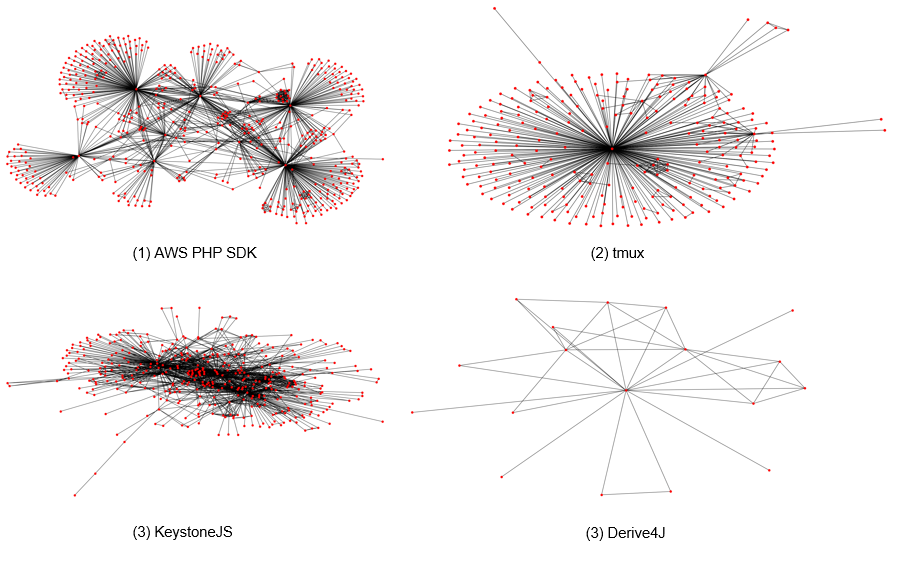
\includegraphics[width=.95\textwidth]{network_plots.PNG}
\caption{Example networks from the data set.}
\label{network_plots}
\end{figure*}

Table \ref{network_summary} shows the summary statistics for each of the network structure variables. For the Gini coefficient, the summary statistics show a tight cluster of stakeholder networks with a moderate level of concentration, contrasted with a smaller number of highly- and lowly-concentrated networks on either end of the distribution. The statistics for average minimum path indicate that most of the stakeholder networks are, per Watts and Strogatz \cite{watts}, relatively small-worlds, although the data set does show substantial variability in the breadth of the networks. The clustering coefficient takes on the most diverse distribution of values, ranging from networks with virtually no localized clustering, such as the network for tmux in Figure \ref{network_structure}, to highly integrated networks, such as the network for KeystoneJS.

\begin{table}
\caption{Summary Statistics for Network Variables}
\label{network_summary}
\begin{tabular}{llllll}
\hline\noalign{\smallskip}
Variable & Min & 25\% & Median & 75\% & Max  \\
\noalign{\smallskip}\hline\noalign{\smallskip}
Gini Coefficient & 0.29 & 0.54 & 0.57 & 0.59 & 0.70 \\
Average Minimum Path & 1.40 & 2.01 & 2.15 & 2.33 & 3.05 \\
Clustering Coefficient & 0.00 & 0.52 & 0.63 & 0.70 & 0.88 \\
\noalign{\smallskip}\hline
\end{tabular}
\end{table}

The scatter plots in Figure \ref{network_structure_scatter} show that crowdsourcing occurs at varying intensities across all network types. The wide distribution of crowdsourcing intensities across network structures makes statistical inference more reliable. Specifically, the distribution allows the models to capture how crowdsourcing interacts with network structure without having to worry about (a) combinations of crowdsourcing and network structure that fall outside the range of observed values in the data set and (b) excessive collinearity between the covariates. This property makes the data set ideal for assessing how network structure impacts the effectiveness of requirements crowdsourcing.

\begin{figure*}
  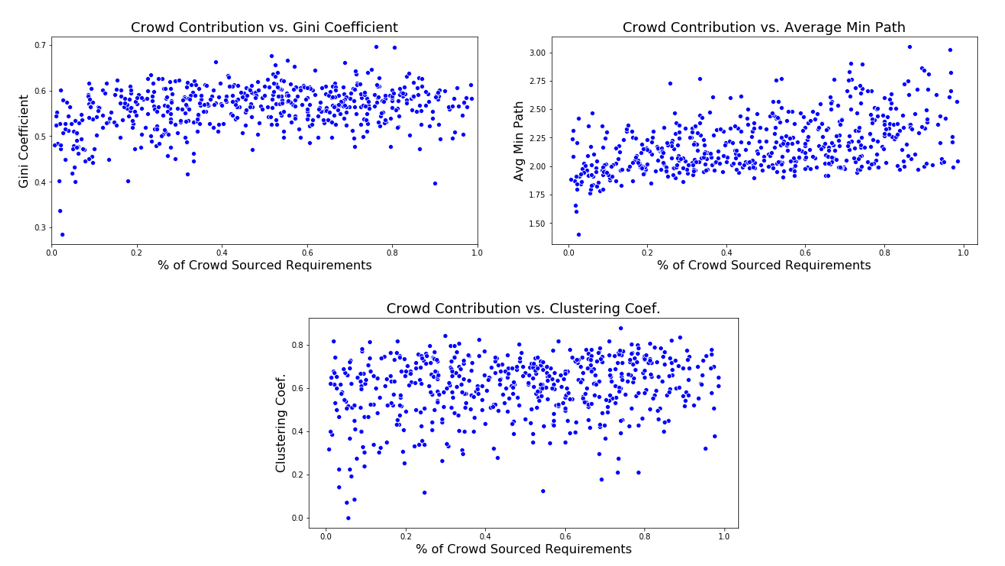
\includegraphics[width=.95\textwidth]{network_structure_scatter.PNG}
\caption{Scatter plots from the input data set.}
\label{network_structure_scatter}
\end{figure*}

\subsection{Regression Results}

\subsubsection{Requirement Close-Out Time}

Within the data set, the average number of days a requirement remains active ranges from less than a day to several years. On average, most projects close out requirements within three months, although the data set does included several projects with very long average close-out times. The results of the KS test fail to reject the null hypothesis that close-out time follows a Gamma distribution, making the Gamma GLM a reasonable model choice.

\begin{figure*}
  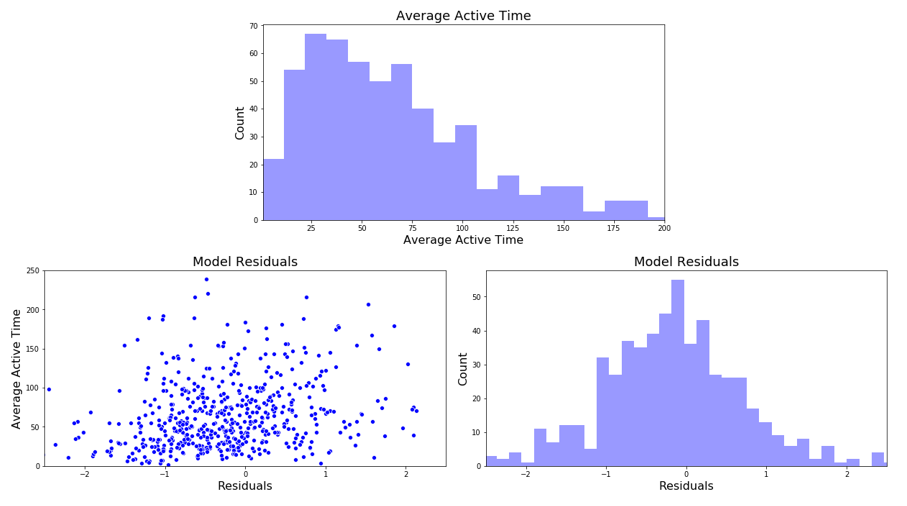
\includegraphics[width=.95\textwidth]{active_time_results.PNG}
\caption{Average requirement close-out time distribution and regression results.}
\label{active_time_results}
\end{figure*}

\begin{figure*}
  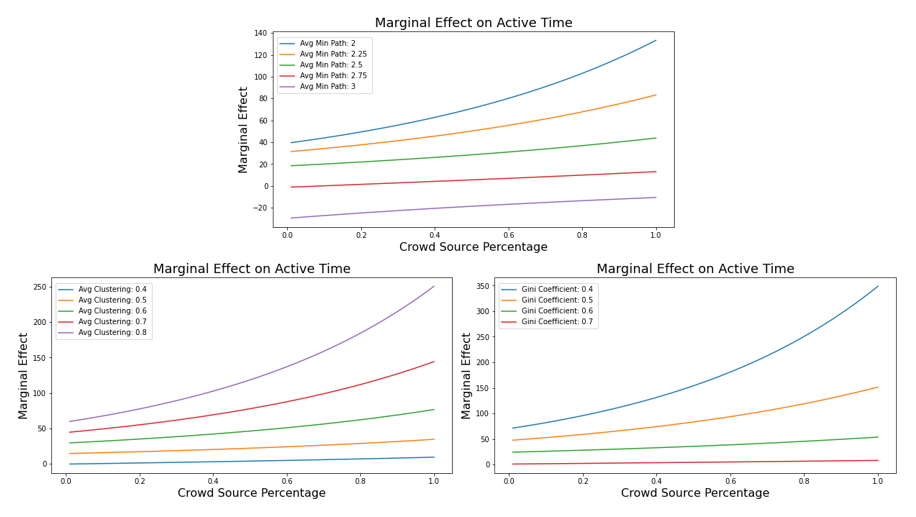
\includegraphics[width=0.95\textwidth]{active_time_marginal.PNG}
\caption{Marginal effects on requirement close-out time as a function of crowdsourcing.}
\label{active_time_marginal}
\end{figure*}

Table \ref{active_time_regression} shows the regression results. All seven variables are statistically significant. The residual plot in Figure \ref{active_time_results} shows no relationship between requirement close-out time and the residuals, which means the results do not raise any concerns about biased estimators.

\begin{table}
\caption{Regression on Requirement Close-out Time}
\label{active_time_regression}
\begin{tabular}{lll}
Gamma GLM | Pseudo $R^2$: 0.51 \\
\hline\noalign{\smallskip}
Variable & Coefficient & p-value  \\
\noalign{\smallskip}\hline\noalign{\smallskip}
Intercept & 0.98 & 0.05 \\
Crowd Percentage & 4.36 & $\leq 0.01$  \\
Average Minimum Path & 0.75 & $\leq 0.01$ \\
Clustering x Crowd Percentage & 3.06 & $\leq 0.01$ \\
Avg Min Path x Crowd Percentage & -1.29 & $\leq 0.01$ \\
Gini Coefficient x Crowd Percentage & -4.75 & $\leq 0.01$ \\
Project Age & 0.0005 & $\leq 0.01$ \\
Nodes & 0.0004 & $\leq 0.01$ \\
\noalign{\smallskip}\hline
\end{tabular}
\end{table}

Figure \ref{active_time_marginal} shows how the marginal effect of increasing the proportion of crowdsourced requirements changes with network structure. For dispersed networks with high concentration and low levels of localized clustering, increasing the share of crowdsourced requirements does not result in substantial increases in requirement close-out time. Networks with the opposite characteristics suffer accelerating requirement close-out times as the share of crowdsourced requirements increases, which indicates that project teams cannot keep up with a growing backlog of crowdsourced requirements. Figure \ref{reqs_contributors_over_time} shows how the total volume of outstanding requirements grows more quickly than the total number of contributors working on the projects. While the figure shows two example projects---KeystoneJS and LeafletJS---the trend holds broadly across the data set. These results point to stakeholder networks with well-defined hubs as a more effective configuration for OSS projects.

\begin{figure*}
  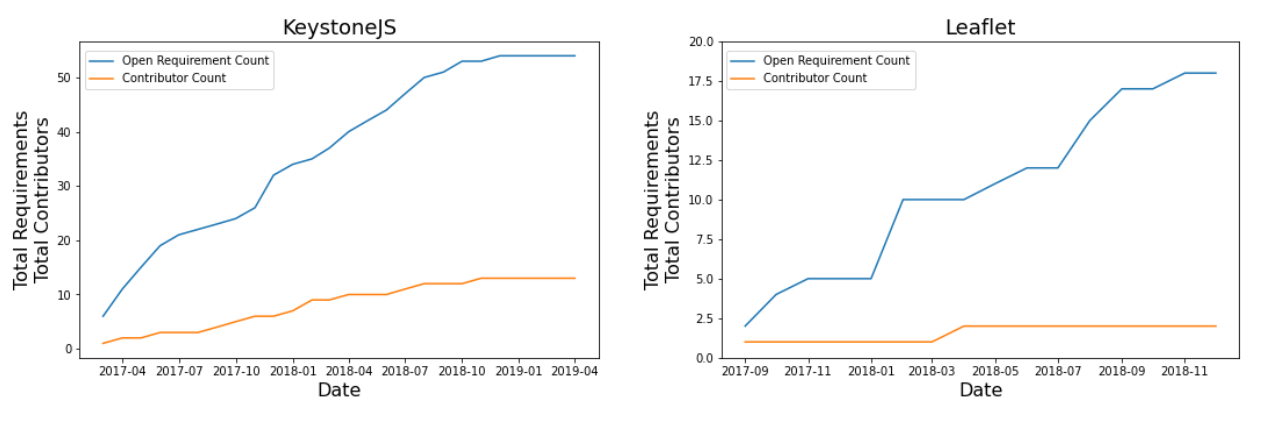
\includegraphics[width=0.95\textwidth]{reqs_contributors_over_time.PNG}
\caption{Open requirements compared to code contributors over time.}
\label{reqs_contributors_over_time}
\end{figure*}

\subsubsection{Requirement Response Time}

The average response times in the data set range from within a day to slightly over a year. As the histogram in Figure \ref{reaction_time_results} shows, the observations follow a lifetime distribution with a long right tail. On average, most projects teams respond to requirements within a month.

\begin{figure*}
  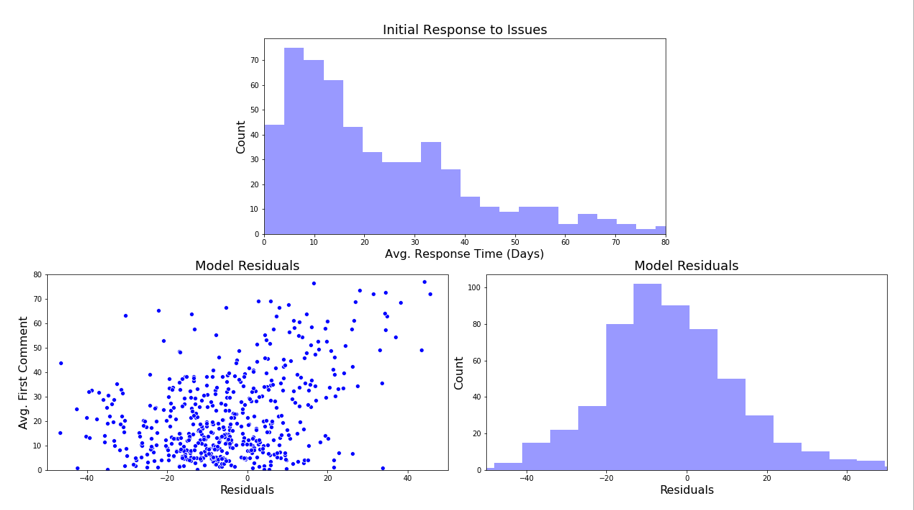
\includegraphics[width=0.95\textwidth]{reaction_time_results.PNG}
\caption{Average requirement response time distribution and regression results}
\label{reaction_time_results}
\end{figure*}

\begin{figure*}
  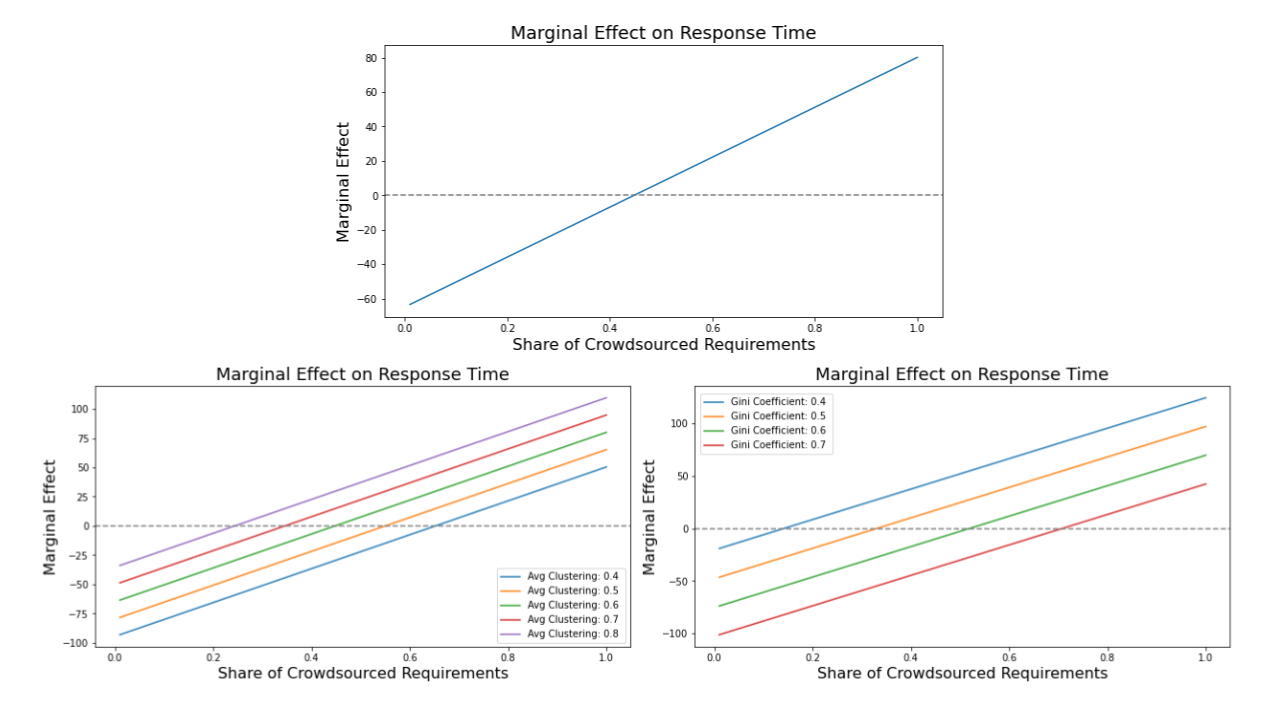
\includegraphics[width=0.95\textwidth]{reaction_time_marginal.PNG}
\caption{Marginal effects on reaction time as a function of crowdsourcing.}
\label{reaction_time_marginal}
\end{figure*}

Table \ref{reaction_time_regression} shows the regression results for requirement response time. For response time, the OLS model had an adjusted $R^2$ of 0.56 compared to a pseudo-$R^2$ of 0.43 for the Gamma GLM. Due to better model performance and because the model appeared to conform to the Gauss-Markov assumptions, the research team opted to use the OLS model. The OLS model includes eight variables, all of which demonstrate statistical significance. As shown in Figure \ref{reaction_time_results}, the residuals approximate a normal distribution and do not correlate with the response variable. Therefore, the model adheres to the Gauss-Markov assumptions \cite{wooldridge} and does not appear likely to suffer from biased estimators.

\begin{table}
\caption{Regression on Response Time}
\label{reaction_time_regression}
\begin{tabular}{lll}
OLS Regression | $R^2$: 0.57 | Adjusted $R^2$: 0.56 \\
\hline\noalign{\smallskip}
Variable & Coefficient & p-value  \\
\noalign{\smallskip}\hline\noalign{\smallskip}
Crowd Percentage Squared & 72.48 & $\leq 0.01$ \\
Gini Coefficient & -69.34 & 0.03 \\
Gini Coefficient X Crowd Percentage & -273.75 & $\leq 0.01$ \\
Clustering Coefficient & -50.78 & 0.03 \\
Clustering Coefficient x Crowd Percentage & 148.08 & $\leq 0.01$ \\
Avg Min Path & 34.13 & $\leq 0.01$ \\
Project Age & 0.02 & $\leq 0.01$ \\
\noalign{\smallskip}\hline
\end{tabular}
\end{table}

The marginal effect plots in Figure \ref{reaction_time_marginal} demonstrate that the impact of requirements crowdsourcing changes dramatically with the structure of the networks. Whereas crowdsourcing a greater share of requirements reduces reaction time for networks with high concentration and low localized clustering, the opposite holds for networks with high localized clustering and low concentration. The direction changes where the marginal effect curves cross zero, switching from negative to positive in Figure \ref{reaction_time_marginal}. Networks with faster response times have a hub-and-spoke structure, suggesting stronger performance for more concentrated stakeholder networks. Moreover, the results show that the marginal impact on response time increases with the share of crowdsourced requirements in the OSS project, which implies that requirements crowdsourcing faces decreasing marginal returns. Overall, these results suggest that OSS project may benefit from either an automated system for prioritizing requirements or a community manager responsible for managing and assigning requirements. These observations reinforce existing results \cite{stakesource, stakerare, lim, mobasher} within the collaborative requirements elicitation literature.

\subsubsection{Comment Activity}
\label{comment_activity}

As noted in Section \ref{measures_of_effectiveness}, average comment activity indicates stronger engagement in the requirements formation process \cite{toral}. Therefore, higher average comment activity represents a positive outcome. Figure \ref{comment_activity_results} includes a histogram showing the distribution of average comments within the data set. The histogram shows that average comment activity has an approximately normal distribution and ranges from 1-8 comments per requirement. While the histogram for comment activity appears normal, since it has a positive domain, modeling comment activity with a Gamma distribution is a reasonable choice. Since the Gamma distribution constitutes a sum of Exponential random variables, the Central Limit Theorem implies that a Gamma distribution can approximate a normal distribution if parameterized properly \cite{wackerly}. Indeed, the results of the KS tests show that the comment activity data fit both the normal and Gamma distributions well under their maximum likelihood estimates. Under these conditions, either a Gamma GLM or an OLS model are sensible options. In this case, the research team favored the Gamma GLM due to materially better model performance.

\begin{figure*}
  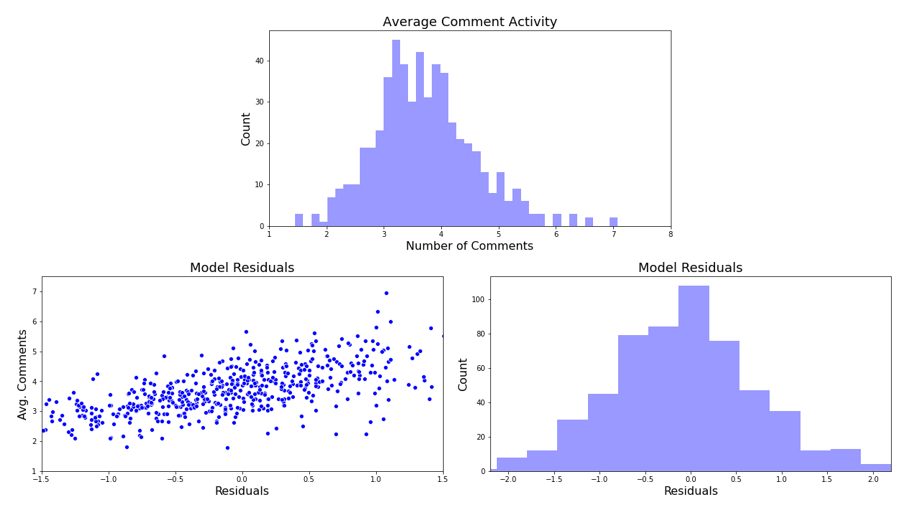
\includegraphics[width=0.95\textwidth]{comment_activity_results.PNG}
\caption{Comment activity distribution and regression results.}
\label{comment_activity_results}
\end{figure*}

\begin{figure*}
  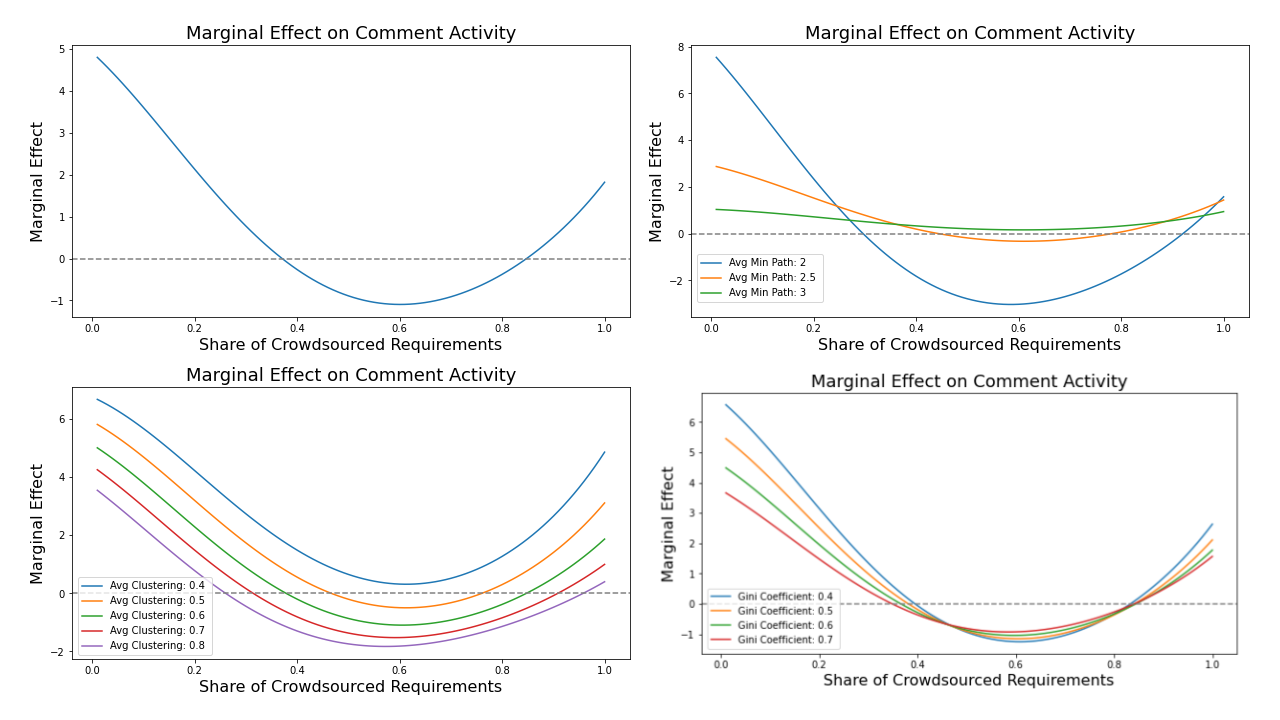
\includegraphics[width=0.95\textwidth]{comment_activity_marginal.PNG}
\caption{Marginal effects on comment activity as a function of crowdsourcing.}
\label{comment_activity_marginal}
\end{figure*}

Table \ref{comment_activity_regression} presents the regression results. Each variable in the regression model is statistically significant. Residual plots for the regression appear in Table \ref{comment_activity_results}. The residual plots show a positive correlation between the residuals and the response variables. However, a linear regression between the dependent variables and the residuals reveals no statistically significant relationship, leading to no concern about biased estimators for this model.

\begin{table}
\caption{Regression on Comment Activity}
\label{comment_activity_regression}
\begin{tabular}{lll}
Gamma GLM | Pseudo $R^2$: 0.46 \\
\hline\noalign{\smallskip}
Variable & Coefficient & p-value  \\
\noalign{\smallskip}\hline\noalign{\smallskip}
Intercept & 0.98 & $\leq 0.01$ \\
Crowd Percentage & 4.10 & $\leq 0.01$ \\
Crowd Percentage Squared & -3.12 & $\leq 0.01$ \\
Crowd Percentage Cubed & 1.69 & $\leq 0.01$ \\
Avg Min Path Squared & 0.35 & $\leq 0.01$ \\
Avg Min Path x Crowd Percentage &  -2.37 & $0.02$ \\
Gini Coefficient Squared & 2.90 & 0.04 \\
Gini Coefficient x Avg Min Path & -2.37 & $\leq 0.01$ \\
Gini Coefficient x Clustering & 5.76 & $\leq 0.01$ \\
Gini Coefficient x Avg Min Path x Crowd Pct & 3.03 & $\leq 0.01$ \\
Gini Coefficient x Clustering Coefficient x Crowd Percentage & -11.24 & $\leq 0.01$ \\
Clustering Coefficient Squared & 1.68 & $\leq 0.01$ \\
Clustering Coefficient x Average Minimum Path & -1.68 & $\leq 0.01$ \\
Clustering Coefficient x Average Minimum Path x Crowd Percentage & 2.12 & $\leq 0.01$ \\
Avg First Comment & -0.002 & $\leq 0.01$ \\
Avg Active Time & 0.001 & $\leq 0.01$ \\
\noalign{\smallskip}\hline
\end{tabular}
\end{table}

The share of crowdsourced requirements and the structure of the stakeholder network have a greater effect on comment activity than on any other measure of effectiveness. The overall trend shows that requirements for OSS projects with very low and very high proportions of crowdsourced requirements generate less discussion than requirements for OSS projects with a moderate share of crowdsourced requirements. Generally, less locally clustered and less concentrated networks generate more comment activity, although the difference for network concentration diminishes for OSS projects with higher proportions of crowdsourced requirements. For dispersed networks, the marginal effect on comment activity remains relatively flat at all levels of crowdsourcing, while networks with a lower average minimum path experience a more pronounced decrease at moderate ranges. Since networks with less localized clustering perform better with respect to comment activity and concentration has a limited effect, these results remain consistent with the hypothesis that stakeholder networks with multiple hubs foster more effective crowd participation in the requirements generation process for OSS projects.

\subsubsection{Contributor Retention Time}

As with comment activity and requirements per crowd member, contributor retention time reflects strong engagement from the crowd. OSS projects benefit by retaining participants for a longer time. The histogram in Figure \ref{reaction_time_results} shows that most crowd members engage with an OSS project for only a few months, although the distribution has a long tail and many crowd members remain engaged for a longer period of time. A KS test on the data shows that, under the maximum likelihood estimates, the response data conforms to a Gamma distribution, making the Gamma GLM a reasonable choice for the regression model. 

\begin{figure*}
  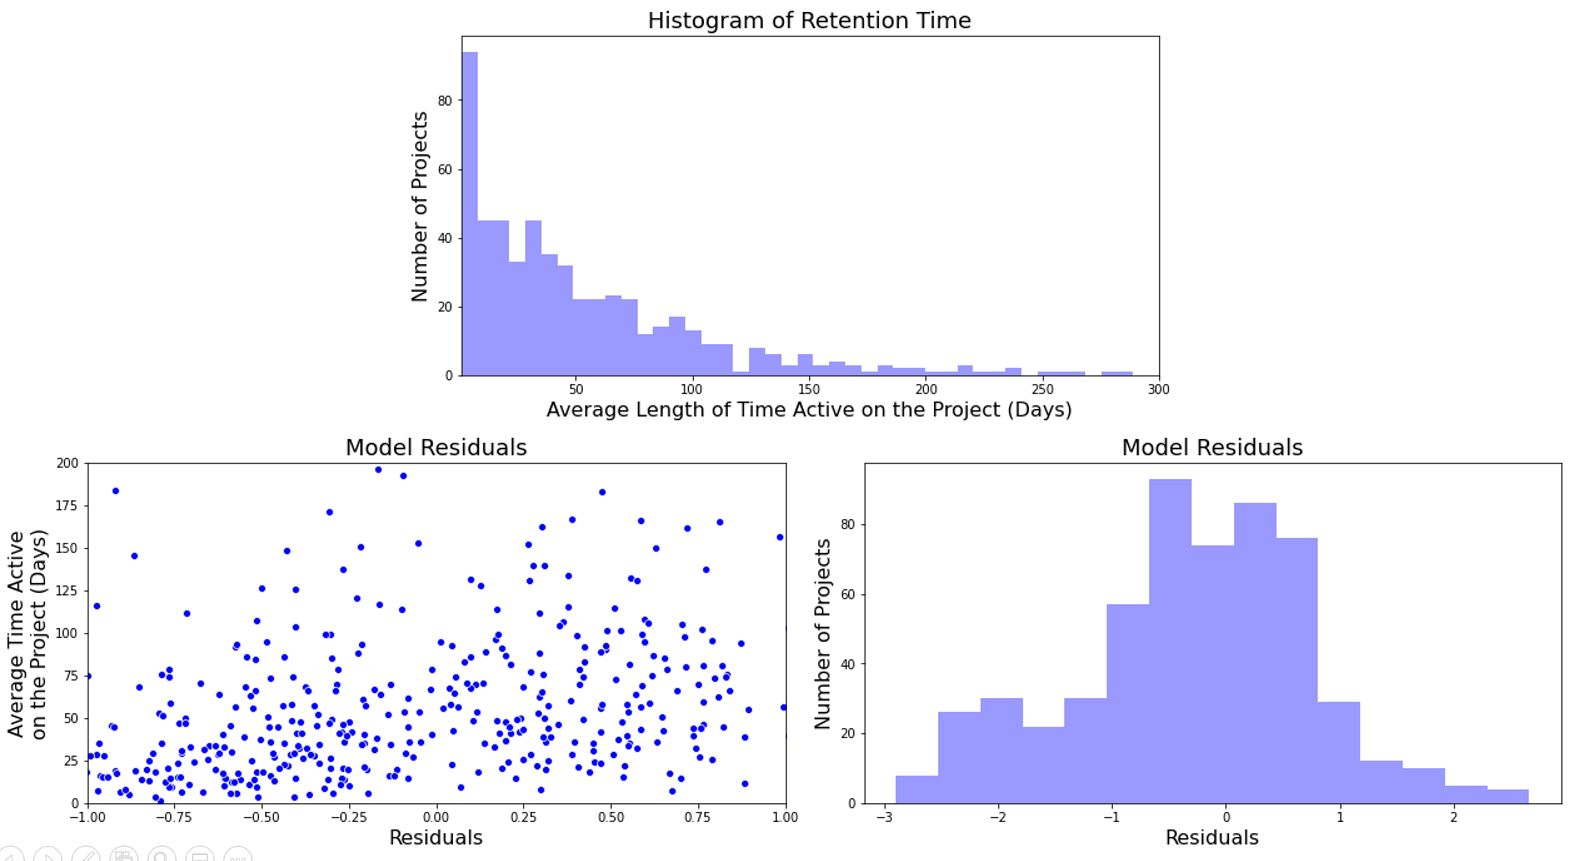
\includegraphics[width=0.95\textwidth]{retention_time_results.PNG}
\caption{Distribution of retention time and regression results.}
\label{retention_time_results}
\end{figure*}

Table \ref{retention_regression} shows the results for the regression. Each variable demonstrates statistical significance. The residual plots, shown in Table \ref{retention_time_results}, show no relationship between the response variables and the residuals, meaning biased estimators do not present a serious concern. A regression of the independent variables against the residuals confirms this assessment.

\begin{table}
\caption{Regression on Retention Time}
\label{retention_regression}
\begin{tabular}{lll}
Gamma GLM | Pseudo $R^2$: 0.42 \\
\hline\noalign{\smallskip}
Variable & Coefficient & p-value  \\
\noalign{\smallskip}\hline\noalign{\smallskip}
Intercept &  4.02 & $\leq 0.01$ \\
Average Minimum Path x Crowd Percentage &  -1.12 & $\leq 0.01$ \\
Average Close-out Time &  -0.0021 &  0.03  \\
Total Open Issues &  0.0011 &  0.01    \\
Project Age &  0.0006 &  $\leq 0.01$    \\
Total Project Contributors &  -0.016 &  $\leq 0.01$ \\
\noalign{\smallskip}\hline
\end{tabular}
\end{table}

Of the network structure variables, only average minimum path had an effect on retention time. The impact of average minimum path on average retention time changes with the share of crowdsourced requirements. Table \ref{reaction_time_marginal} shows the marginal effect on average retention time of an increase in the proportion of crowdsourced requirements. Under all conditions, an increasing the share of crowdsourced requirements decreases average retention time, although the magnitude of the effect diminishes once an OSS project crowdsources a higher proportion of requirements. While additional crowdsourcing has a less detrimental effect on OSS projects with less dispersed stakeholder networks, network structure ceases to have a major impact once a project sources more than 40\% of requirements from the crowd. The results of this regression confirm concerns in the CrowdRE literature \cite{glinz, groen, levy} about maintaining motivation in large crowds and suggests OSS projects could benefit from adopting CrowdRE methods such as gamification. 

\begin{figure*}
  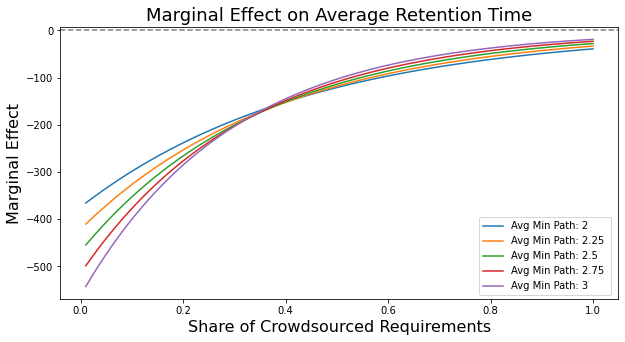
\includegraphics[width=0.95\textwidth]{retention_time_marginal.PNG}
\caption{Marginal effects on retention time as a function of crowdsourcing.}
\label{retention_time_marginal}
\end{figure*}

\subsubsection{Requirements Per Crowd Member}

The average number of requirements per crowd member measures the intensity of engagement between the project team and the crowd. Multiple requirement submissions by a single crowd member signals strong engagement and represents a positive outcome for an OSS project. As shown in Figure \ref{requirements_per_user_results}, for most projects, each crowd member submits relatively few requirements. However, the distribution has a long right tail, and some projects average several dozen requirements per crowd member. The results of the KS test validate that the variable conforms to a Gamma distribution, per the assumptions of the Gamma GLM.

\begin{figure*}
  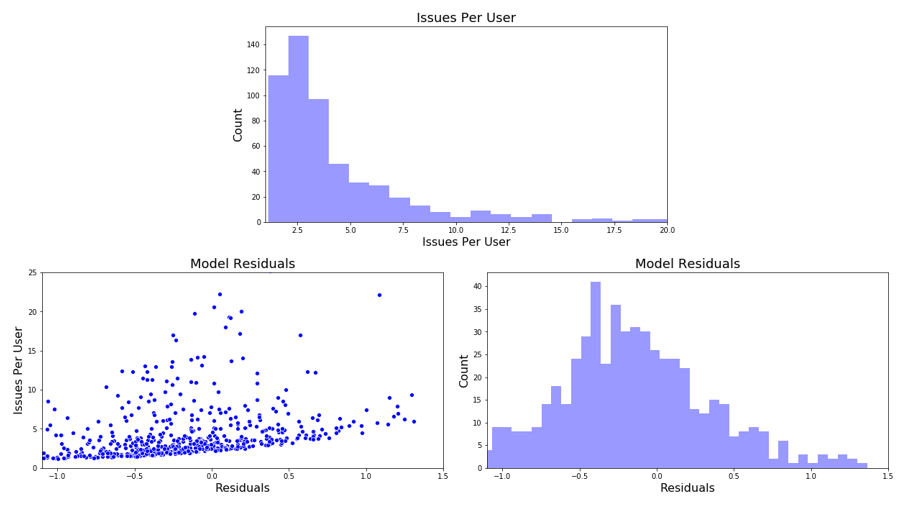
\includegraphics[width=0.95\textwidth]{issues_per_user_results.PNG}
\caption{Distribution of requirements per crowd member and regression results.}
\label{requirements_per_user_results}
\end{figure*}

\begin{table}
\caption{Regression on Requirements Per Crowd Member}
\label{requirements_per_user_regression}
\begin{tabular}{lll}
Gamma GLM | Pseudo $R^2$: 0.64 \\
\hline\noalign{\smallskip}
Variable & Coefficient & p-value  \\
\noalign{\smallskip}\hline\noalign{\smallskip}
Intercept & 2.17 & $\leq 0.01$ \\
Crowd Percentage & -7.90 & $\leq 0.01$ \\
Crowd Percentage Squared & 6.40 & $\leq 0.01$  \\
Average Minimum Path & 0.52 & $\leq 0.01$  \\
\noalign{\smallskip}\hline
\end{tabular}
\end{table}

The regression results for the network and requirements crowdsourcing variables appear in Table \ref{requirements_per_user_regression}. In contrast to the other measures of effectiveness, the variable selection process only selected a small number of regressors for this model. The model includes three variables, each of which demonstrates statistical significance. Of the network structure variables, only average minimum path appears in the equation. Its effect, however, does not change with the share of crowdsourced requirements. Other network structure variables do not have a statistically significant effect when included in the regression. This leads to the conclusion that, while the proportion of crowdsourced requirements affects the number of requirements per crowd member, the effect does not change with the structure of the stakeholder network. 

Figure \ref{requirements_per_user_results} shows a positive correlation between requirements per crowd member and the residuals. A linear regression of the residuals against the dependent variables shows a slight positive correlation between crowd percentage and the residuals, and a slight negative correlation between crowd percentage squared and the residuals. These results imply bias toward zero for both of the coefficients, meaning the model probably overestimates the effect of crowdsourcing. However, the base and squared crowdsourcing terms both have roughly the same coefficient in the residual regression, meaning the positive-to-negative crossover point remains unbiased, even though the GLM overestimates the overall effect of crowdsourcing.

The coefficients indicate that additional crowdsourcing decreases the number of requirements per crowd member for projects that source less that 65\% of their requirements from the crowd, and increases the number of requirements per crowd member beyond that threshold. Combining this observation with the crowd retention results from the previous section produces interesting insights. For OSS projects with a high share of crowdsourced requirements, increasing crowd participation in the requirements generation process both reduces the average retention time for crowd members and increases the expected number of requirements per crowd member. This implies that, for OSS projects that source a substantial share of requirements from the crowd, most of those requirements come from a relatively small number of highly engaged crowd members. Without recruiting and motivating crowd members beyond that core group, OSS projects may miss out on some of the benefits of requirements crowdsourcing, including the discovery of novel use cases.

\subsubsection{Requirement Volume}

Requirement volume measures the total number of requirements, scaled by the age of the project in years. The histogram in Figure \ref{requirement_volume_results} shows that the distribution of requirement volume in the data set follows a lifetime distribution with a long right tail, with a maximum value of 84 requirements per year. KS test results show that requirement volume follows a Gamma distribution, justifying the choice to employ a Gamma GLM model. The CrowdRE literature \cite{groen} recognizes that a higher volume of requirements produces trade-offs for a project team. While more feedback enables the team to understand user perceptions of an OSS project, the ability to maintain task completion velocity as crowd participation grows presents serious concerns. Additionally, too much feedback leads to `featuritis' \cite{glinz}, making work difficult to prioritize. Therefore, a complete analysis of this variable must include an assessment of the trade-off between requirement volume and other measures of effectiveness.

\begin{figure*}
  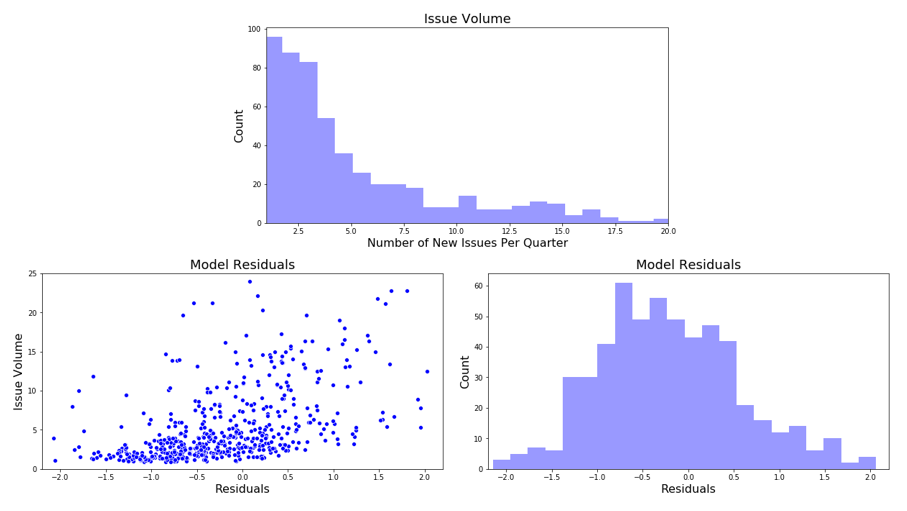
\includegraphics[width=0.95\textwidth]{issue_volume_results.PNG}
\caption{Requirement volume distribution and regression results.}
\label{requirement_volume_results}
\end{figure*}

\begin{figure*}
  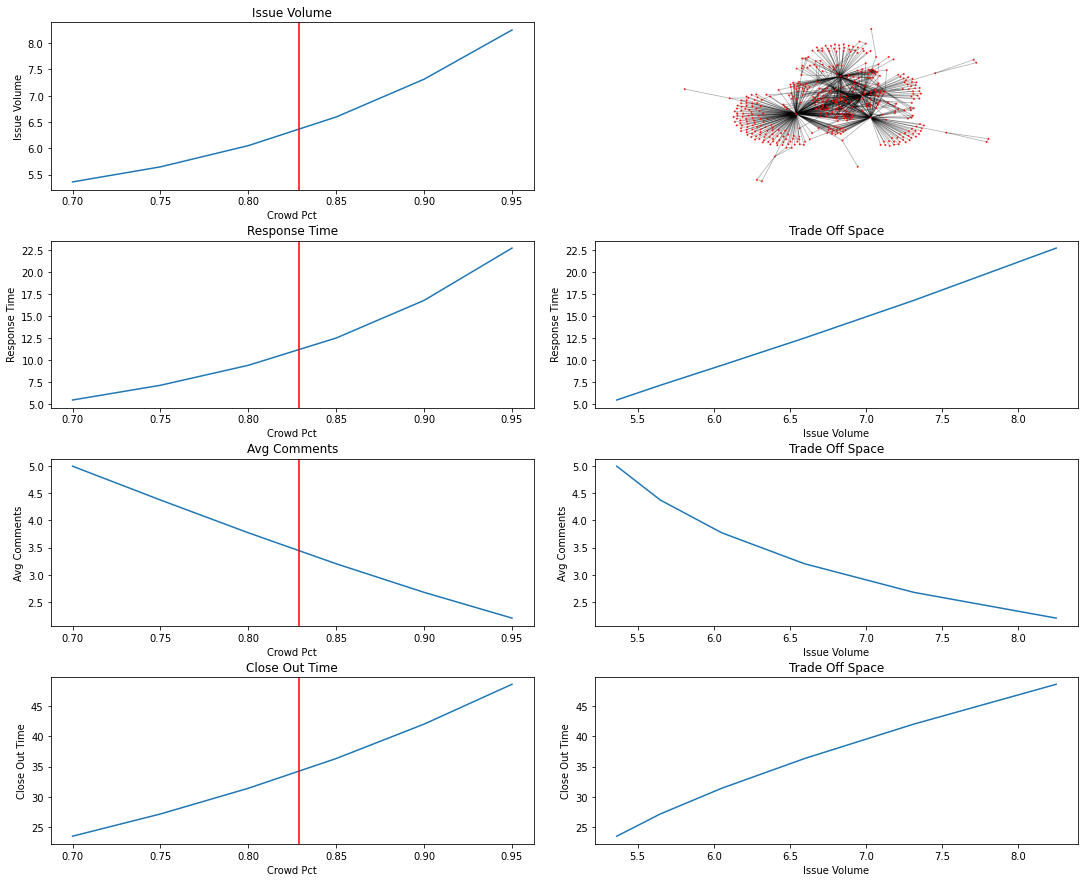
\includegraphics[width=0.95\textwidth]{leaflet_trade_space.png}
\caption{Trade-off space as requirement volume increase for LeafletJS.}
\label{leaflet_trade_space}
\end{figure*}

The regression results for the GLM appear in Table \ref{requirement_volume_regression}. Each variable in the model is statistically significant. As opposed to the results for the other measures of effectiveness, the effect of additional crowdsourcing of requirement volume does not change with network structure. While higher network concentration does promote higher issue volume, the effect is independent of the level of crowdsourcing.  The residual plot in Figure \ref{requirement_volume_results} shows slight positive correlation between the residuals and requirement volume. However, a linear regression of the residuals against the dependent variable does not show any correlation, which means the regression does not have biased estimators. As show in Figure \ref{issue_volume_marginal}, the effect of crowdsourcing additional requirements is negative when the current share of crowdsourced requirements is below 70\%, at which point the effect of additional requirements crowdsourcing becomes positive.

\begin{table}
\caption{Regression on Requirement Volume}
\label{requirement_volume_regression}
\begin{tabular}{lll}
Gamma GLM | Pseudo $R^2$: 0.54 \\
\hline\noalign{\smallskip}
Variable & Coefficient & p-value  \\
\noalign{\smallskip}\hline\noalign{\smallskip}
Intercept & 1.39 & $\leq 0.01$ \\
Crowd Percentage &  -5.01 & $\leq 0.01$  \\
Crowd Percentage Squared & 3.69 & $\leq 0.01$  \\
Gini Coefficient & 3.87 & $\leq 0.01$  \\
Total Contributors & 0.02 & $\leq 0.01$ \\
Total Users & 0.01 & $\leq 0.01$ \\
\noalign{\smallskip}\hline
\end{tabular}
\end{table}

\begin{figure*}
  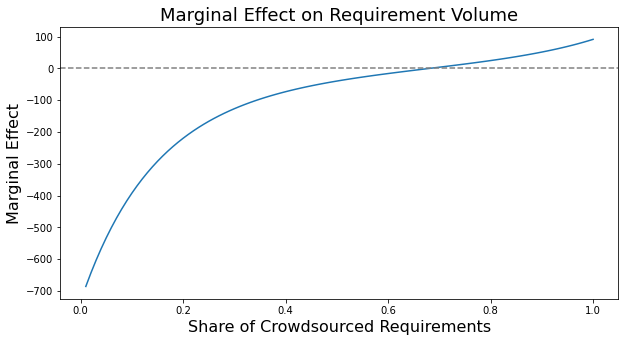
\includegraphics[width=0.95\textwidth]{issue_volume_marginal.PNG}
\caption{Marginal effects on requirement volume as a function of crowdsourcing.}
\label{requirement_volume_marginal}
\end{figure*}

As noted in Section \ref{measures_of_effectiveness}, an increase in requirement volume can represent a positive or a negative outcome, depending on the circumstances. project managers can determine the costs and benefits of an increase in requirement volume by plotting the trade-off space between requirement volume and other measures of effectiveness. Figure \ref{leaflet_trade_space} shows the trade-off analysis for LeafletJS, a JavaScript geospatial library. In this example, an increase in requirement volume results in longer response and close-out times and less comment activity on each requirement, reflecting a trade-off between levels of crowd engagement and the comprehensiveness of the requirement set. The trade-off plots suggest the presence of two phenomena. First, growing crowd sizes result in social loafing, whereby crowd members comment less actively on requirements in the expectation that other members of the crowd will pick up the slack. Second, the increase in close-out time may reflect the need to validate and clarify more complex uses cases, which arise due to feedback from a more diverse set of stakeholders. In addition to requirements elicitation, these trade-offs imply that project managers should engage with the crowd to validate and prioritize requirements. Collaborative requirements elicitation techniques \cite{stakerare, mobasher} can aid in that endeavor. At certain levels of engagement, projects may benefit more from validating existing requirements than from sourcing new ones. Trade-off plots provide project managers with the ability to make an informed decision based on the circumstances specific to a project.

\section{Conclusion}

\subsection{Summary}

This work employed regression models to analyze the impact of network structure and requirements crowdsourcing on the performance of OSS projects with respect to six measures of effectiveness. The results support each of the three hypotheses outlined in Section \ref{intro}.

Requirement close-out time and requirement response time indicate the level of engagement and productivity of the project team. The regression results show that, under most circumstances, crowdsourcing a greater share of requirements increases the amount of time it takes to close out requirements. Figure \ref{reqs_contributors_over_time} demonstrates the reason for this phenomenon: the volume of open requirements increases faster than the size of a project team over time, leading to a growing backlog of unaddressed requirements. OSS projects whose stakeholder networks have hub-and-spoke structures better contend with this challenge, with requirement close-out time remaining close to flat under the most ideal circumstances.

While crowdsourcing always increases close-out time, the effect on requirement response time varies based on the stakeholder network structure and the current share of crowdsourced requirements. For projects that crowdsource a small share of requirements, and increase in the proportion of crowdsourced requirements decreases requirement response time. Conversely, additional crowdsourcing increases requirement response time for OSS projects that currently crowdsource a high proportion of requirements. The crossover point occurs at the 30-70\% mark, depending on the stakeholder networks structure, and occurs later for more concentrated stakeholder networks. This fortifies the notion that OSS projects benefit from having organized and concentrated stakeholder networks and lends support to the micro-crowd strategy Levy, Hadar, and Te'eni \cite{levy} propose for building engagement from small, highly connected groups of users.

Requirement comment activity, contributor retention time, and requirements per crowd member measure levels of crowd engagement. Comment activity follows an unusual pattern in that additional requirements crowdsourcing lowers comment activity for OSS projects that currently source a very small or very large proportion of requirements from the crowd. For OSS projects that source a moderate share of requirements from the crowd, crowdsourcing additional requirements decreases comment activity, except for highly concentrated networks. For these networks, the marginal effect on comment activity decreases at moderate proportions of requirements crowdsourcing, but never turns negative. Again, this supports the argument that more concentrated networks promote better performance.

Increasing the share of crowdsourced requirements reduces the average retention time of crowd members. This holds at all values for the current share of crowdsourced requirements, although the effect decreases as the share of crowdsourced requirements increases. While OSS projects with less dispersed stakeholder networks observe a smaller decrease in retention time, the difference disappears for projects that source more than 40\% of requirements from the crowd. For OSS projects that currently crowdsource a small share of requirements from the crowd, an increase in crowdsourcing reduces the average requirements per crowd member. The average requirements per crowd member, however, increases with the proportion of crowdsourced requirements for OSS projects that already generate most of their requirements from the crowd. Taken together, the results for retention time and requirements per crowd member lead to the conclusion that, for OSS projects that crowdsource a large proportion of requirements, most of the requirements originate from a small set of highly active crowd members. 

Finally, the results for requirements volume show that increases in the share of crowdsourced requirements results in a lower volume of requirements for OSS projects that generate a limited number of requirements from the crowd. For OSS projects that crowdsource a substantial portion of requirements, the effect flips, meaning that crowdsourcing a greater share of requirements results in a higher requirement volume. Stakeholder networks with higher levels of concentration tend to have higher requirement volumes. Since increasing the volume of requirements does not reflect an unambiguously good or bad outcome, trade-off analysis enables OSS project managers to understand the impact of encouraging the crowd to submit more requirements.

\subsection{Discussion}

This research adds to the existing literature in crowdsourcing and CrowdRE, for several reasons. First, the analysis presents a novel application of CrowdRE within an OSS context. In his review of the state of CrowdRE, Glinz \cite{glinz} highlights the lack of CrowdRE applications for OSS requirements generation as a research gap. This research both utilizes CrowdRE to assess the impact of stakeholder network structure and requirements crowdsourcing on OSS project performance and develops a CrowdRE approach OSS project managers can use to determine the best strategy for engaging with the crowd.

Second, the results suggest that, beyond a certain threshold, crowdsourcing additional requirements can hurt an OSS project more than it helps. For OSS projects that already crowdsource more than about 70\% of requirements, increasing the share of crowdsourced requirements results in longer requirement close-out and response times, a growing backlog of unaddressed requirements, and shorter retention time for crowd members. These factors reinforce one another. A higher volume of requirements increases average requirement close-out time, which in turn lowers the crowd retention rate.

Third, this paper suggests that OSS project managers need to consider not only how to incentive crowd participation, but also when. The discussion in the previous paragraph does not imply that project managers should discourage requirements crowdsourcing, even when they already crowdsource a sizable share of requirements. Rather, once an OSS project already crowdsources a substantial portion of requirements, project managers should focus instead on prioritizing existing requirements by applying the collaborative requirements elicitation techniques outlined in Section \ref{network_re}.

Fourth, this research shows that stakeholder network structure has a significant effect on outcomes for OSS projects, and that the impact of stakeholder network structure changes depending on the proportion of requirements a project crowdsources. The results show that more concentrated stakeholder networks perform better across multiple measures of effectiveness. Highly concentrated hub-and-spoke networks correlate with shorter requirement close-out and response times and higher comment activity on requirements. In addition to validating existing research by Iyer and Lyytinen \cite{iyer} and Toral, et al. \cite{toral}, this research expands the current understanding of the topic by showing that the effect of network structure changes with the share of crowdsourced requirements, utilizing multiple network structure variables, and considering additional measures of effectiveness.

Finally, this paper uses empirical analysis to verify several claims from the CrowdRE literature. First, the surprising conclusion that average comment activity increases for projects with a high share of crowdsourced requirements even as the total volume of requirements grows suggests that crowd engagement succeeds in surfacing new perspectives. Groen et al. \cite{groen} claims gathering perspectives from a more diverse range of stakeholders as one of the main benefits of crowd engagement. Furthermore, the results showing lower retention when an OSS projects crowdsources a larger share of requirements validates concerns within the \mbox{CrowdRE} literature \cite{snijders, snijders2, levy} about maintaining crowd motivation, and suggests applying CrowdRE techniques could help. Additionally, the observation that increases in requirement close-out times lower crowd retention supports Groen, et al.'s \cite{groen} assertion that crowds often include impact seekers, whose motivation depends on the implementation of their suggestions. All of this reinforces the notion that the crowd represents an important construct for thinking about the requirements process for OSS projects.

This paper also has important practical implications. Most importantly, it suggests both that OSS project teams can benefit from using CrowdRE tools, and that the decision on which tool to use depends on the current state of the project. If projects that have stakeholder networks with hub-and-spoke structures produce better outcomes, project managers can benefit from implementing strategies to encourage the formation of these structures. Hub-and-spoke networks result from direct interaction between a crowd member and the appropriate member of the project team. Natural language tools such as Mobasher's \cite{mobasher} recommendation system that identifies the appropriate implementer based on the content of a requirement could help promote such connections. Assigning a project team member to engage with crowd members and route requirements could also result in more efficient patterns of engagement between team members and the crowd.

This work suggests that OSS project teams must employ different CrowdRE tools depending on the current level of requirements crowdsourcing for the project. If a project currently crowdsources a small share of requirements, OSS project managers would benefit from gamification techniques \cite{snijders, snijders2} that incentivize additional crowd participation. Once a project crowdsources a substantial share of requirements, OSS project managers should focus on collaborative elicitation techniques for routing and prioritizing requirements.

\subsection{Limitations and Threats to Validity}
\label{limitations}

While this paper develops useful insights, readers should keep in mind several limitations and threats to validity.

\subsubsection{Limitations}

First, this research only considers software. Physical products present different challenges because they have longer feedback cycles and less mutable specifications. Moreover, while the data set covers a broad range of OSS projects, it only includes active, widely adopted packages. The results may not apply equally well to smaller OSS packages with less active user bases. Additionally, as Scacchi \cite{scacchi} notes, proprietary software and corporate-led OSS projects follow more formal procedures for requirements gathering and development. Because of these differences, the results in this paper do not apply to software projects in more structured settings.

Second, the OSS projects in the data set target developers as the user base. This presents several challenges. On average, since they come from the software development community, OSS and GitHub users have unusually strong technical skills. Therefore, they can formulate technical requirements without needing a product manager as an intermediary. These conditions do not hold for consumer-facing OSS projects, such as web-applications. Users of consumer-facing tools more commonly express the need for a particular feature, which a product manager translates into a technical requirement that the development team can implement. Due to the specialized nature of the crowds in the data set, the results in this paper do not generalized beyond OSS projects with a technical audience.

Third, this research only considers requirements elicitation for existing software. Consequently, the software projects in the data set have already advanced beyond the design phase. Formulating requirements for new software involves more uncertainty and necessarily benefits less from crowd participation because software does not have any users at the onset. Furthermore, crowd members have less incentive to participate in the requirements process because they do not yet actively rely on the software as a dependency. Therefore, the results in this research only apply to OSS projects that have advanced beyond the design phase.

Fourth, the CrowdRE literature typically considers a selective, well-moderated crowd \cite{stakerare}. Research by Lim \cite{stakerare, stakesource, lim} and others which indicates that crowd engagement results in higher quality requirements does not extend automatically to unmoderated crowds of OSS contributors. Assessing the impact of unmoderated crowd contributions on requirement quality necessitates further research.

Fifth, this research only considers the requirements generation process. It does not consider other components of the requirements process, such as validation and prioritization. As such, this research does not shed additional light on Lim, et al.'s \cite{stakenet} conclusion that a high volume of crowd-generated requirements biases prioritization in favor of more active stakeholders.

Finally, the analysis does not capture every measure of effectiveness for OSS projects in the existing literature. Specifically, this study omits product quality \cite{stewart}, project team satisfaction \cite{ghapanchi}, user satisfaction \cite{ghapanchi}, requirement quality \cite{ma}, and the extent to which the crowd agrees about the content and relatively importance of requirements \cite{ma}. 

\subsubsection{Threats to Validity}

This research also faces a number of threats to validity. First, this research does not account for project complexity. Project complexity could impact the results because more complex projects increase the amount of time team members need to implement requirements and create a barrier to entry for crowd members to generate reasonably high quality requirements. Factors such as the number of lines of code, the number of modules, and the extent to which the modules interact within one another could serve as a proxy for project complexity

Second, this research assumes that different types of software projects have the same optimal network structure. In reality, low-level systems software might require higher levels of specialized expertise, and therefore benefit from a different patterns of crowd interaction than a web-development framework, which has a broader user base. 

Finally, the research assumes static stakeholder networks. In reality, stakeholder network structure changes over time as new developers join or leave. A core developer leaving a project could alter the structure of the stakeholder network quite dramatically. This presents less of a concern for this data set than for OSS projects more broadly because the data consists of a curated set of active projects. However, accounting for temporal dynamics in the stakeholder networks would make the analysis more robust and more broadly applicable.

\subsection{Future Research}

This research prompts several questions that could serve as the basis for follow-on research. First, this study shows that longer requirement close-out times lead to greater crowd attrition in the aggregate. Future research could evaluate this phenomenon at the individual contributor level by observing whether or not the implementation of a crowd member's requirement impacts the probability that the crowd member submits another requirement in the future.

Second, the results in this paper indicate that more concentrated stakeholder networks produce better outcomes for OSS projects. A reasonable hypothesis to explain this phenomenon is that each hub is a contributor who specializes in a particular aspect of the code base. These stakeholder networks may perform better as crowdsourcing expands because each contributor only needs to focus on a small subset of incoming requirements. An investigation to determine whether different hubs in these networks indeed specialize based on requirement type could yield valuable insights.

Third, one of the proposed benefits of CrowdRE is that it leads to the generation of new requirements that project managers would not have identified if they had not solicited feedback from the crowd. If crowd members and project team members produce similar requirements, that would negate this benefit. A research effort to determine the degree to which crowd-generated requirements differ from internally sourced requirements could help shed light on this issue.

Fourth, as suggested in Section \ref{trade-off}, future research could develop more sophisticated models to analyze the trade-off space between various measures of effectiveness. These models should account for the change in network structure that occurs when OSS projects source additional requirements from the crowd, and include sensitivity analysis that quantifies how a change in network structure would impact the trade-off space.

Fifth, future work could consider different types of crowds and requirements process activities. The results, for instance, may not hold for crowds with less technical acumen. Crowdsourcing for other requirements process activities, such as validation and prioritization, may likewise benefit from different patterns of engagement. 

Sixth, future research could consider aspects of an OSS project, such as requirement quality and project complexity, that this research did not consider. These variables present challenges due to the inability to directly measure them from the data. Measuring these variables would likely requiring training an additional predictive model, which would add uncertainty to the analysis.

Finally, this study considers stakeholder networks as a snapshot in time. In reality, the structure of these networks evolves along with their their performance characteristics. An effort to study how these stakeholder networks arrived at their current structure could help project managers design interventions that will guide their interactions with the crowd toward a positive outcome. Additional, future research could address how various types of developer interactions correlate with the evolution of network structure over time.

\subsection{Summary}

This study used a GitHub data set consisting of project management artifacts from a curated set of 562 open-source software projects to evaluate the impact of stakeholder network structure on the effectiveness of crowd-based requirements processes. The results supports each of the hypotheses in Section \ref{intro}. For five out of six measures of effectiveness, statistical analysis shows that the marginal impact of additional crowdsourcing changes with the structure of the stakeholder network and the current proportion of crowdsourced requirements. The results suggest that OSS projects whose stakeholder networks have hub-and-spoke structures perform better as the proportion of crowdsourced requirements increases. These structures result from direct engagement on requirements between crowd members and the appropriate member of the project team. OSS project managers can promote the development of stakeholder networks with hub-and-spoke structures by adopting CrowdRE strategies that route crowdsourced requirements based on their content.

The results also show that requirements crowdsourcing faces diminishing marginal returns as the proportion of crowdsourced requirements increases. In particular, crowdsourcing more than about 70\% of requirements results in longer requirement close-out and response times, a higher volume of open requirements, and shorter average retention times for crowd members. As such, beyond that threshold, OSS project members would benefit more from channeling existing crowd engagement than from incentivizing crowd members to submit additional requirements. While this research establishes a relationship between stakeholder network structure, the share of crowdsourced requirements, and measures of effectiveness for OSS projects, the results do not generalize to OSS projects with less technical users, proprietary software, or physical products.

 \section*{Conflict of interest}

The authors declare that they have no conflict of interest.

\section*{Availability of data and material}

Data is available at BLINDED.

\section*{Code availability}

Code is available at BLINDED.

\section*{Author contributions}

The material in this paper has been abstracted and developed from a dissertation submitted to the BLINDED in partial fulfillment of the requirements for BLINDED's Ph.D. degree.

\begin{thebibliography}{}

\bibitem{anscombe}
Anscombe, FJ, \& Tukey, JW (1963) The examination and analysis of residuals. Technometrics, 5(2): 141-160.

\bibitem{brabham}
Brabham, D (2013) Crowdsourcing. MIT Press, Cambridge.

\bibitem{brabham2}
Brabham, D (2008) Crowdsourcing as a odel for problem solving: An introduction and cases 14(1): 75-90.

\bibitem{camara}
Camara, G \& Fonseca, F (2007) Information policies and open source software in developing countries. Journal of the American society for information science and technology, 58(1): 121-132.

\bibitem{javascript}
Chen, C. Awesome JavaScript, GitHub Repository, https://github.com/sorrycc/awesome-javascript (2019)

\bibitem{python}
Chen, V (2019) Awesome Python GitHub Repository. https://github.com/vinta/awesome-python Accessed 15 June 2019

\bibitem{crowston}
Crowston, K \& Howison, J (2016) FLOSS Project Effectiveness Measures. Successful OSS Project Design and Implementation: Requirements, Tools, Social Designs and Reward Structures: 149.

\bibitem{damian}
Damian, D, Marczak, S, \& Kwan, I (2007) Collaboration patterns and the impact of distance on awareness in requirements-centred social networks. In 15th IEEE International Requirements Engineering Conference (RE 2007): 59-68.

\bibitem{derkson}
Derksen, S, \& Keselman, HJ (1992) Backward, forward and stepwise automated subset selection algorithms: Frequency of obtaining authentic and noise variables. British Journal of Mathematical and Statistical Psychology, 45(2): 265-282.

\bibitem{fahrmeir}
Fahrmeir, L, Kneib, T, Lang, S, \& Marx, B (2007) Regression. Springer-Verlag Berlin, Heidelberg: 300-301.

\bibitem{cpp}
Fallahi, F, (2019) Awesome C++ GitHub Repository. https://github.com/fffaraz/awesome-cpp Accessed 15 June 2019

\bibitem{finkelstein}
Finkelstein, A (1994) Requirements Engineering: a review and research agenda. In Proceedings of 1st Asia-Pacific Software Engineering Conference: 10-19.

\bibitem{ferrari}
Ferrari, S, \& Cribari-Neto, F (2004) Beta regression for modelling rates and proportions. Journal of applied statistics, 31(7): 799-815.

\bibitem{friedman}
Friedman, J, Hastie, T, \& Tibshirani, R (2001) The elements of statistical learning (Vol. 1, No. 10). Springer series in statistics, New York: 60-61.

\bibitem{ghapanchi}
Ghapanchi, A , Aurum, A, \& Low, G (2011) A taxonomy for measuring the success of open source software projects. First Monday.

\bibitem{gerth}
Gerth, RJ, Burnap, A, \& Papalambros, P (2012) Crowdsourcing: A primer and its implications for project managering. Michigan University, Ann Arbor.

\bibitem{gini}
Gini, C (1912) Variabilità e mutabilità. Reprinted in Memorie di metodologica statistica (Ed. Pizetti E, Salvemini, T). Libreria Eredi Virgilio Veschi, Rome.

\bibitem{gini2}
Gini, C (1921) Measurement of inequality of incomes. The Economic Journal, 31(121): 124-126.

\bibitem{glinz}
Glinz, C (2019) CrowdRE: Achievements, Opportunities and Pitfalls. Proc. REW 2019. 

\bibitem{groen}
Groen, EC, Seyff, N, Ali, R, Dalpiaz, F, Doerr, J, Guzman, E, ... \& Stade, M (2017) The crowd in requirements engineering: The landscape and challenges. IEEE software, 34(2): 44-52.

\bibitem{holland}
Holland, PW, \& Leinhardt, S (1971) Transitivity in structural models of small groups. Comparative group studies, 2(2): 107-124.

\bibitem{howe2}
Howe, J (2008) Crowdsourcing: How the power of the crowd is driving the future of business. Random House.

\bibitem{howe}
Howe, J (2006) The rise of crowdsourcing, Wired magazine 14, no. 6: 1-4.

\bibitem{hosseini}
Hosseini, M, Phalp, KT, Taylor, J, \& Ali, R (2014) Towards crowdsourcing for requirements engineering.

\bibitem{incose}
INCOSE.Systems Engineering Handbook: A Guide for System Life Cycle Processes and Activities, Fourth Edition. Wiley, 2015

\bibitem{iyer}
Iyer, DG and Lyytinen, K (2019). "REQUIREMENTS ENGINEERING (RE) EFFECTIVENESS IN OPEN SOURCE SOFTWARE: THE ROLE OF SOCIAL NETWORK CONFIGURATIONS AND REQUIREMENTS PROPERTIES". In Proceedings of the 27th European Conference on Information Systems (ECIS), Stockholm \& Uppsala, Sweden, June 8-14, 2019.

\bibitem{kuriakose}
Kuriakose, J \& Parsons, J (2015) How do open source software (OSS) developers practice and perceive requirements engineering? An empirical study. In 2015 IEEE Fifth International Workshop on Empirical Requirements Engineering (EmpiRE). IEEE: 49-56

\bibitem{java}
Kull, A (2019) Awesome Java GitHub Repository. https://github.com/akullpp/awesome-java Accessed 15 June 2019.

\bibitem{khan}
Khan, JA, Liu, L, Wen, L \& Ali, R (2019) Crowd Intelligence in Requirements Engineering: Current Status and Future Directions, Proc. REFSQ 2019, LNCS 11412: 45-261.

\bibitem{kluender}
Kluender, J, Schneider, K, Kortum, F, Straube, J, Handke, L, \& Kauffeld, S (2016) Communication in teams-an expression of social conflicts. In Human-Centered and Error-Resilient Systems Development: 111-129.

\bibitem{latoza}
LaToza, TD, \& Van Der Hoek, A (2015) Crowdsourcing in software engineering: Models, motivations, and challenges. IEEE software, 33(1): 74-80.

\bibitem{levy}
Levy, M., Hadar, I., \& Te'eni, D.,. A gradual approach to crowd-based requirements engineering: The case of conference online social networks, 2015 IEEE 1st International Workshop on Crowd-Based Requirements Engineering (CrowdRE), 25-30, IEEE (2015)

\bibitem{stakerare}
Lim, SL, \& Finkelstein, A (2011) StakeRare: using social networks and collaborative filtering for large-scale requirements elicitation. IEEE transactions on software engineering, 38(3): 707-735.

\bibitem{stakenet}
Lim, SL, Quercia, D, \& Finkelstein, A (2010) StakeNet: using social networks to analyse the stakeholders of large-scale software projects. In 2010 ACM/IEEE 32nd International Conference on Software Engineering, Vol. 1: 295-304.

\bibitem{stakesource}
Lim, SL, Quercia, D, \& Finkelstein, A (2010) StakeSource: harnessing the power of crowdsourcing and social networks in stakeholder analysis. In 2010 ACM/IEEE 32nd International Conference on Software Engineering, Vol. 2.

\bibitem{lim}
Lim, SL, \& Ncube, C (2013) Social networks and crowdsourcing for stakeholder analysis in system of systems projects. In 2013 8th International Conference on System of project managering: 13-18.

\bibitem{linaker}
Linåker, J, Regnell, B, \& Damian, D (2020) A method for analyzing stakeholders’ influence on an open source software ecosystem’s requirements engineering process. Requirements Engineering, 25(1): 115-130.

\bibitem{lopez}
Lopez-Fernandez, L, Robles, G, \& Gonzalez-Barahona, J (2004) Applying Social Network Analysis to the Information in CVS Repositories. MSR. Vol. 2004.

\bibitem{ma}
Ma, Q (2009) The effectiveness of requirements prioritization techniques for a medium to large number of requirements: a systematic literature review (Doctoral dissertation, Auckland University of Technology).

\bibitem{mao}
Mao, K, Capra, L, Harman, M, \& Jia, Y (2017) A survey of the use of crowdsourcing in software engineering. Journal of Systems and Software, 126: 57-84.

\bibitem{massey}
Massey Jr, FJ (1951) The Kolmogorov-Smirnov test for goodness of fit. Journal of the American statistical Association, 46(253): 68-78.

\bibitem{missonier}
Missonier, S, \& Loufrani-Fedida, S (2014) Stakeholder analysis and engagement in projects: From stakeholder relational perspective to stakeholder relational ontology. International Journal of Project Management, 32(7): 1108-1122.

\bibitem{mitchell}
Mitchell, RK, Agle, BR, \& Wood, DJ (1997) Toward a theory of stakeholder identification and salience: Defining the principle of who and what really counts. Academy of management review, 22(4): 853-886.

\bibitem{mobasher}
Mobasher, B. \& Cleland-Huang, J (2011) Recommender Systems in Requirements Engineering, AI Magazine, vol. 32, no. 3: 81-89.

\bibitem{newcombe}
Newcombe, R (2003) From client to project stakeholders: a stakeholder mapping approach. Construction management and economics, 21(8): 841-848.

\bibitem{paech}
Paech, B. \& Reuschenbach, B (2006) Open source requirements engineering. In 14th IEEE International Requirements Engineering Conference (RE'06) IEEE: 257-262.

\bibitem{pagano}
Pagano, D \& Maalej, W. (2013) User Feedback in the AppStore: An Empirical Study, in Proc. RE 2013: 125-134.

\bibitem{parnell}
Parnell, GS (2016) Trade-off analytics: creating and exploring the system tradespace. John Wiley \& Sons.

\bibitem{regnell}
Regnell, B \& Brinkkemper, S. (2005) Market-driven requirements engineering for software products. In Engineering and managing software requirements. Springer, Berlin, Heidelberg: 287-308.

\bibitem{robinson}
Robinson, W, \& Vlas, R (2015) Requirements evolution and project success: an analysis of SourceForge projects.


\bibitem{scacchi}
Scacchi, W (2009) Understanding requirements for open source software. Design requirements engineering: A ten-year perspective. Springer, Berlin, Heidelberg: 467-494.

\bibitem{sen}
Sen, A, Sen, \& Foster, JE (1997) On economic inequality. Oxford University Press, Oxford.

\bibitem{setia}
Setia P, Rajagopalan B, Sambamurthy V, Calantone R (2012) How peripheral developers contribute to open-source software development. Information Systems Research, 23(1): 144-163.

\bibitem{sharp}
Sharp, H, Finkelstein, A, \& Galal, G (1999). Stakeholder identification in the requirements engineering process. In Proceedings. Tenth International Workshop on Database and Expert Systems Applications. DEXA 99: 387-391.

\bibitem{snijders}
Snijders, R, Dalpiaz, F, Hosseini, M, Shahri, A, \& Ali, R (2014) Crowd-centric requirements engineering. In 2014 IEEE/ACM 7th International Conference on Utility and Cloud Computing: 614-615.

\bibitem{snijders2}
Snijders, R, Atilla, O, Dalpiaz, F, \& Brinkkemper, S (2015) Crowd-Centric Requirements Engineering: A method based on crowdsourcing and gamification. Technical Report Series, (UU-CS-2015-004).

\bibitem{stewart}
Stewart, KJ \& Gosain, S (2006) The impact of ideology on effectiveness in open source software development teams. MIS Quarterly: 291-314.

\bibitem{stol}
Stol, KJ, LaToza, TD, \& Bird, C (2017) Crowdsourcing for software engineering. IEEE software, 34(2): 30-36.

\bibitem{toral}
Toral, SL, Martínez-Torres, MDR, \& Barrero, F (2010) Analysis of virtual communities supporting OSS projects using social network analysis. Information and Software Technology, 52(3): 296-303.

\bibitem{ullman}
Ullman, JB, \& Bentler, PM (2003) Structural equation modeling. Handbook of psychology: 607-634.

\bibitem{veall}
Veall, MR, \& Zimmermann, KF (1996) Pseudo‐R2 measures for some common limited dependent variable models. Journal of Economic surveys, 10(3): 241-259.

\bibitem{wackerly}
Wackerly, D, Mendenhall, W, \& Scheaffer, RL (2014) Mathematical statistics with applications. Cengage Learning: 477-485.

\bibitem{watts}
Watts, DJ, \& Strogatz, SH (1998) Collective dynamics of ‘small-world’ networks. nature, 393(6684): 440.

\bibitem{wang}
Wang, C, Daneva, M.,  van Sinderen, M \& Liang, P (2019) A Systematic Mapping Study on Crowdsourced Requirements Engineering using User Feedback, J Softw. Evol. Proc., vol. 31, no. 10.

\bibitem{wood}
Wood, J, Sarkani, S, Mazzuchi, T, \& Eveleigh, T (2013) A framework for capturing the hidden stakeholder system. Systems Engineering, 16(3): 251-266.

\bibitem{wooldridge}
Wooldridge, JM (2015) Introductory econometrics: A modern approach: Nelson Education. Scarborough, ON, Canada: 60-62.

\bibitem{yitzhaki}
Yitzhaki, S (1979) Relative deprivation and the Gini coefficient. The quarterly journal of economics: 321-324.

\bibitem{php}
York, J (2019) Awesome PHP GitHub Repository. https://github.com/ziadoz/awesome-php Accessed 15 June 2019.

\end{thebibliography}

\section*{Appendix}

\subsection*{Edge Direction in Stakeholder Networks}

Using undirected, unweighted graphs follows a pattern established in most of the studies cited in Section \ref{network_re}. Weighted edges provide an advantage insofar as they allow the model to capture the intensity of the relationship between stakeholders. Toral, Martinez-Torres, and Barrero \cite{toral}, for instance, use weighted edges to study the influence of knowledge brokers within networks and argue that more frequent interactions indicates a more robust connection between stakeholders. The network models in this research do not include weights because, for some metrics, their inclusion produces counter-intuitive results. Higher edge weights, for instance, typically reflect longer distances between nodes, whereas more frequent interactions should reduce the distance between stakeholders. Edge weights do improve fidelity for centrality measures, such as the edge degree of nodes. However, weighting would also reduce the variability of concentration measurements within the data set, making statistical inference more difficult. Given the methodological difficulty involved in incorporating edge weights and the limited potential benefit, the research team decided to use unweighted edges.

Toral, Martinez-Torres, and Barrero \cite{toral} use directed edges to represent information flow within their networks. Specifically, they use discussion threads as the primary unit of analysis and construct networks that represent a directed chain of replies. Within the context of their work, directed edges add value due to their ability to model information flows. In the current study, however, networks represent spontaneous two-way collaborations rather than a series of replies, meaning undirected edges have a more intuitive interpretation. As a result, the research team decided to construct the stakeholder networks using undirected edges.

\subsection*{Additional Notes on the Gini Coefficient}

Using the Gini coefficient to measure concentration in stakeholder networks resultings in some interesting properties. In particular, the value of the Gini coefficient \cite{gini, gini2} for the degree distribution of nodes in a network cannot reach one because every edge connects to a pair of nodes. As a result, a single node cannot collect degrees without sharing degrees with other nodes. As a result, the maximum value for the Gini coefficient for a network grows with the number of nodes, but never reaches one. Similarly, the effective lower bound of the Gini coefficient for networks remains above zero. Although this property makes the Gini coefficient an imperfect measure of network concentration, as a practical matter, it only impacts relatively small networks.

The original formulation defines the Gini coefficient using the Lorenz curve \cite{gini}. However, Sen provides an equivalent formulation, which calculates the Gini coefficient as half the mean absolute difference \cite{sen}. This formulation appears in Equation \ref{gini_coef}. Due to its simplicity, the research team decided to compute the Gini coefficient using the Sen formulation.

\begin{equation}
\label{gini_coef}
    G = \frac{\sum_{i=1}^{n} \sum_{j=i}^{n} | x_{i} - x{j} |}{2n^2 \bar{x}}
\end{equation}

\end{document}